\iffalse \bibliography{MGymrekRefs.bib} \fi

\chapter{lobSTR: A short tandem repeat profiler for personal genomes}

\hzline

Most of this chapter was first published as:

\begin{itemize}
\item[] \textbf{Gymrek M}, Golan D, Rosset S, Erlich Y. lobSTR: a short tandem repeat profiler for personal genomes. \emph{Genome Research}. (2012).
\item[] \textbf{Gymrek M}, Erlich Y. Profiling short tandem repeats from short reads. Book chapter in \emph{Deep Sequencing Data Analysis} by \emph{Methods Mol Biol} (2013).
\end{itemize}

Part of this work is covered by a U.S. patent:

\begin{itemize}
\item[] Analyzing short tandem repeats from high throughput sequencing data for genetic applications. (2013). Inventors: Erlich Y, \textbf{Gymrek M}. US 2014/0163900 A1.
\end{itemize}

\hzline

\textbf{Abstract}: Short Tandem Repeats (STRs) have a wide range of applications, including medical genetics, forensics, and genetic genealogy. High throughput sequencing (HTS) has the potential to profile hundreds of thousands of STR loci. However, mainstream bioinformatics pipelines are inadequate for the task. These pipelines treat STR mapping as gapped alignment, which results in cumbersome processing times and a biased sampling of STR alleles. Here, we present lobSTR, a novel method for profiling STRs in personal genomes. lobSTR harnesses concepts from signal processing and statistical learning to avoid gapped alignment and to address the specific noise patterns in STR calling. The speed and reliability of lobSTR exceed the performance of current mainstream algorithms for STR profiling. We validated lobSTR's accuracy by measuring its consistency in calling STRs from whole genome sequencing of two biological replicates from the same individual, by tracing Mendelian inheritance patterns in STR alleles in whole-genome sequencing of a HapMap trio, and by comparing lobSTR results to traditional molecular techniques. Encouraged by the speed and accuracy of lobSTR, we used the algorithm to conduct a comprehensive survey of STR variations in a deeply sequenced personal genome. We traced the mutation dynamics of close to 100,000 STR loci and observed more than 50,000 STR variations in a single genome. lobSTR's implementation is an end-to-end solution. The package accepts raw sequencing reads and provides the user with the genotyping results. It is written in C/C++, includes multi-threading capabilities, and is compatible with the BAM format.

lobSTR is available at \url{https://github.com/mgymrek/lobstr-code}.

\section{Introduction}
Short tandem repeats (STRs), also known as microsatellites, are a class of genetic variations with repetitive elements of 2 to 6 nucleotides that consists of approximately a quarter million loci in the human genome \cite{Benson1999}. The repetitive structure of those loci creates unusual secondary DNA conformations that are prone to replication slippage events and result in high variability in the number of repeat elements \cite{Mirkin2007}. The spontaneous mutation rate of STRs exceeds that of any other type of known genetic variation, and can reach 1/500 mutations per locus per generation \cite{Walsh2001,BallantyneGoedbloedFangEtAl2010}, 200 fold higher than the rate of spontaneous copy number variations (CNV) \cite{Lupski2007} and 200,000 fold higher than the rate of de novo SNPs \cite{ConradKeeblerDePristoEtAl2011}.

STR variations have been instrumental in wide-ranging areas of human genetics. STR expansions are implicated in the etiology of a variety of genetic disorders, such as Huntington's Disease and Fragile-X Syndrome \cite{PearsonNicholEdamuraCleary2005,Mirkin2007}. Forensics DNA-fingerprinting relies on profiling autosomal STR markers and Y-chromosome STR (Y-STR) loci \cite{KayserKnijff2011}. STRs have been extensively used in genetic anthropology, where their high mutation rates create a unique capability to link recent historical events to DNA variations, including the well-known Cohen Modal Haplotype that segregates in patrilineal lines of Jewish priests \cite{SkoreckiSeligBlazerEtAl1997,ZhivotovskyUnderhillCinniogluEtAl2004}. Another relatively recent application of STR analysis is tracing cell lineages in cancer samples \cite{FrumkinWasserstromItzkovitzEtAl2008}.

Despite the plurality of applications, STR variations are not routinely analyzed in whole genome sequencing studies, mainly due to a lack of adequate tools \cite{TreangenSalzberg2012}. STRs pose a remarkable challenge to mainstream HTS analysis pipelines. First, not all reads that align to an STR locus are informative (\textbf{Supplemental Figure~\ref{fig:lobsup1}A}). If a single or paired-end read partially encompasses an STR locus, it provides only a lower bound on the number of repeats. Only reads that fully encompass an STR can be used for exact STR allelotyping. Second, mainstream aligners, such as BWA, generally exhibit a trade-off between run time and tolerance to insertions/deletions (indels) \cite{LiHomer2010}. Thus, profiling STR variations -- even for an expansion of three repeats in a trinucleotide STR -- would require a cumbersome gapped alignment step and lengthy processing times (\textbf{Supplemental Figure~\ref{fig:lobsup1}B}). Third, PCR amplification of an STR locus can create stutter noise, in which the DNA amplicons show false repeat lengths due to successive slippage events of DNA polymerase during amplification \cite{HaugeLitt1993,Ellegren2004} (\textbf{Supplemental Figure~\ref{fig:lobsup1}C}). Since PCR amplification is a standard step in library preparation for whole genome sequencing, an STR profiler should explicitly model and attempt to remove this noise to enhance accuracy.

Here, we present lobSTR, a rapid and accurate algorithm for STR profiling in whole genome sequencing datasets (\textbf{Figure \ref{fig:lobfig1}}). Briefly, the algorithm has three steps. The first step is sensing: lobSTR swiftly scans genomic libraries, flags informative reads that fully encompass STR loci, and characterizes their STR sequence. This ab initio procedure relies on a signal processing approach that uses rapid entropy measurements to find informative STR reads followed by a Fast Fourier Transform to characterize the repeat sequence. The second step is alignment: lobSTR uses a divide and conquer strategy that anchors the non-repetitive flanking regions of STR reads to the genome to reveal the STR position and length. We use a modified reference that takes advantage of the information extracted from the sensing step to increase the alignment specificity. This step avoids a cumbersome gapped alignment and, importantly, is virtually indifferent to the magnitude of STR variations. Finally, in the third step, the pipeline allelotypes the STRs using a statistical learning approach that models the stutter noise in order to enhance the signal of the true allelic configuration. See \textbf{Supplemental Text \ref{sec:lobsupptext}}, \textbf{Supplemental Figures \ref{fig:lobsup2}, \ref{fig:lobsup3}, \ref{fig:lobsup4}, \ref{fig:lobsup5}} and \textbf{Supplemental Table \ref{tab:lobsuptab1}} for full details about the lobSTR algorithm.

\begin{figure}[h!]
\centering
\label{fig:lobfig1}
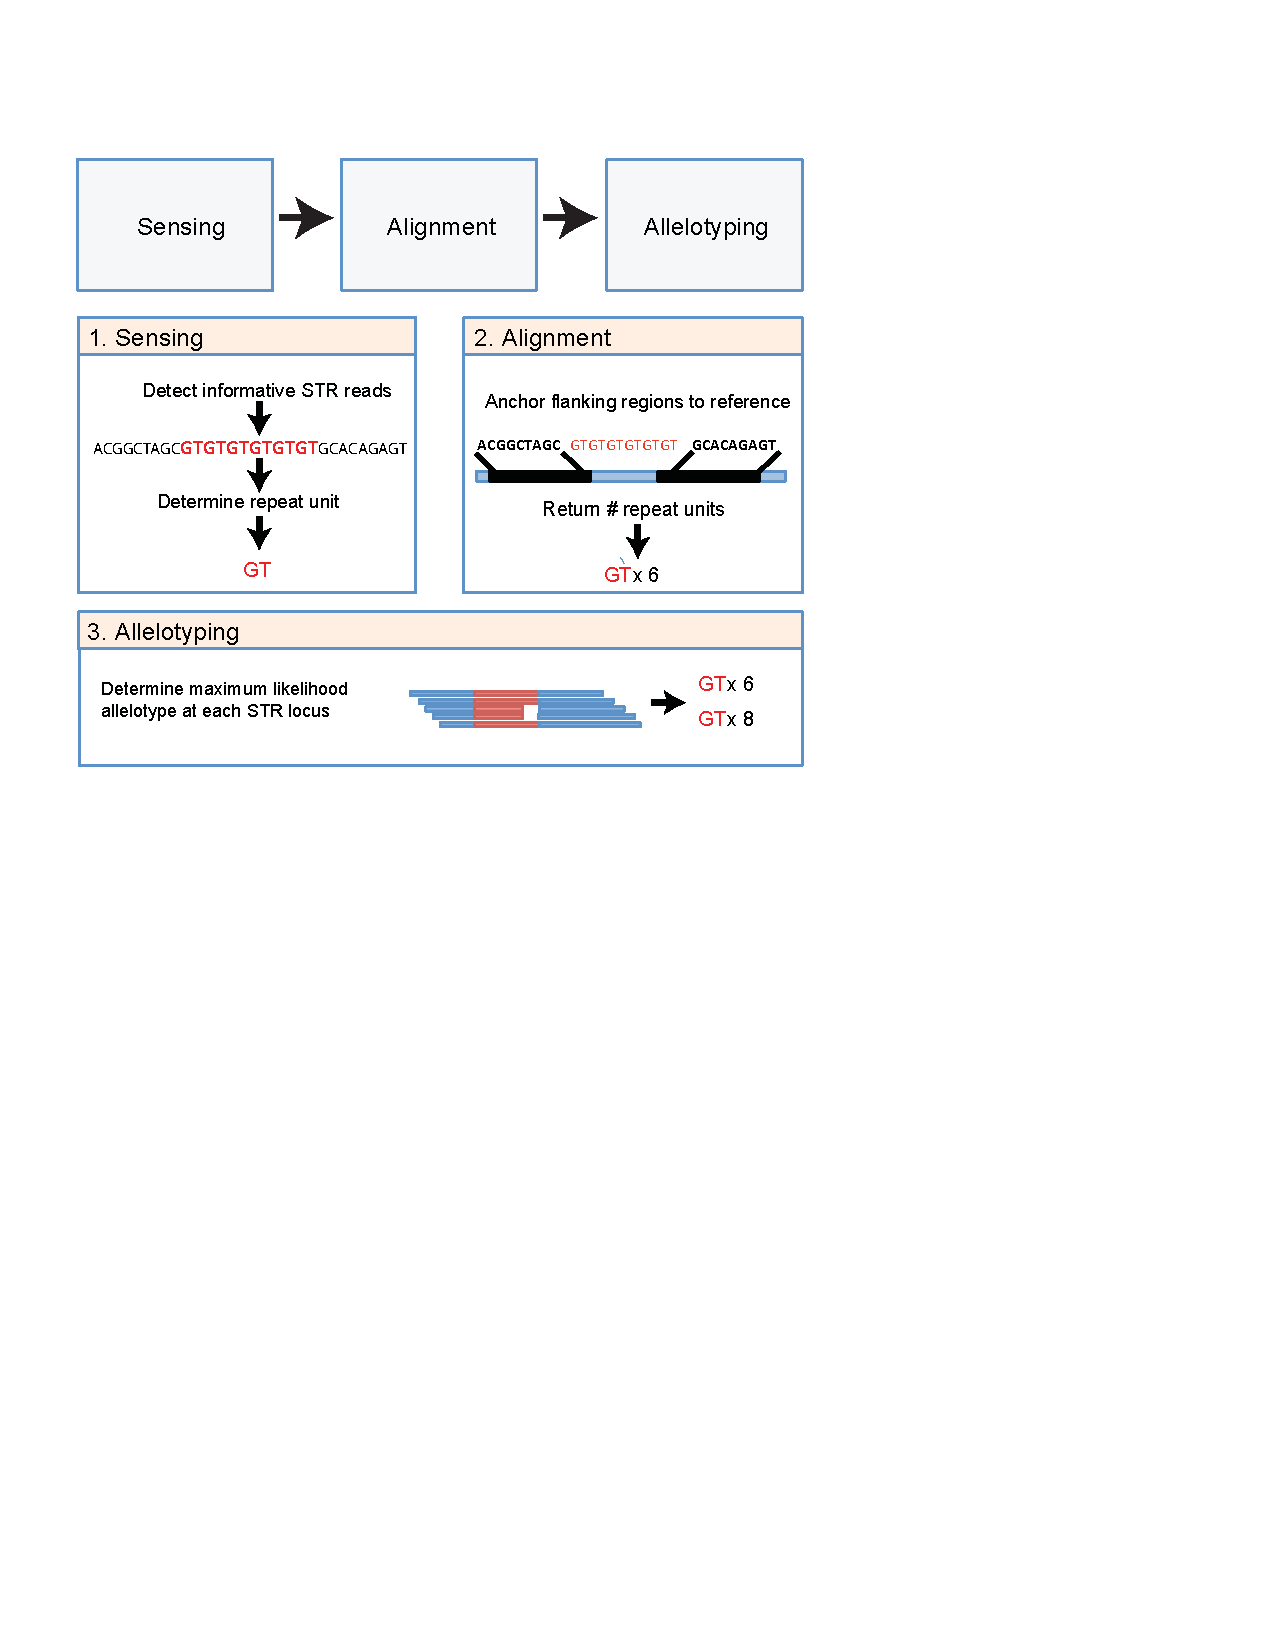
\includegraphics[width=0.5\textwidth]{Figures/Chapter2/Fig1.pdf}
\caption{\textbf{lobSTR algorithm overview} lobSTR consists of three steps. The sensing step detects informative STR reads and determines their repeat motif. The alignment step maps the STRs' flanking regions to the reference. The allelotyping step determines the STR alleles present at each locus.}
\end{figure}

lobSTR implementation offers a complete solution that takes raw sequencing data and reports the alleles present at each profiled STR locus. The program's input is one or more sequencing libraries in FASTA/FASTQ or BAM format. The output is the alignment of STR reads in BAM format and the most likely alleles for each STR locus in a custom tab-delimited text format. lobSTR supports multi-threaded processing.

\section{Results}
\subsection{Comparing lobSTR to mainstream aligners}

We benchmarked lobSTR's alignment performance with reads from an Illumina whole genome sequencing library with 101bp reads (\textbf{Methods \ref{sec:lobmethods}}). To demonstrate its added value for STR profiling over mainstream aligners, we also ran BWA, Novoalign, and Bowtie on the same input data with and without the GATK local indel realignment tool. In addition, we ran BLAT \cite{Kent2002} to characterize STR alignment by a tool that is centered on sensitivity rather than speed. BWA and Novoalign were tested with the default parameters that can detect up to 5bp and 7bp indels, respectively. Bowtie has no indel tolerance and was evaluated as a control condition with tolerance of up to two mismatches. BLAT was tested with the default parameters that can tolerate up to 10\% divergence from the reference, which corresponds to approximately 10bp indels. To focus on the pure algorithm speed-up, all tests were executed on a single CPU.

lobSTR excelled in all the parameters required for efficient STR alignment (\textbf{Table \ref{tab:lobtab1}}). First, lobSTR processed the reads 2.2 times faster than Bowtie, 22 times faster than BWA, 70 times faster than Novoalign, and almost 1000 times faster than BLAT (\textbf{Figure \ref{fig:lobfig2}A}). These results indicate that there is a minimal computational payment in running lobSTR in parallel to mainstream aligners in order to augment variation calling to include STR polymorphisms. Second, as required, lobSTR reported only informative reads that fully encompass STR loci. On the other hand, the mainstream aligners reported between 2,000 to 5,000 non-informative STR reads per million input sequences, which may confound downstream calling algorithms if not removed. Third, lobSTR detected the largest number of informative reads with STR variations compared to mainstream aligners (\textbf{Figure \ref{fig:lobfig2}B}). The other aligners showed a strong tendency to report STR reads with the reference allele vis-a-vis with their indel tolerance. Bowtie did not report any STR variation. After GATK local realignment, BWA and Novoalign, respectively, reported that 20\% and 25\% of the informative reads have STR variations. BLAT reported that 37\% of the informative reads have STR variations, compared to 50\% in lobSTR. Analyzing data collected from a large number of randomly ascertained STR loci \cite{PayseurJingHaasl2011} (Utah Marker Development Group) demonstrates that 33-66\% of STR sequence reads should exhibit a non-reference allele (see Methods). This suggests that lobSTR's results are more representative of the true rate of STR variations than mainstream alignment tools.

\begin{table}[h!]
\centering
\label{tab:lobtab1}
\begin{adjustbox}{width=1\textwidth}
\begin{tabular}{l l l l l l l l}
\hline
Algorithm & Indel tolerance (bp) & Time (sec)& \# Non-informative reads & \# Informative reads & \# Var. reads$^a$	& Ratio$^b$ & Peak memory (Gbyte) \\
\hline
lobSTR & - & 109 & 0 & 973 & 485 & 0.5 & 0.3\\
Bowtie&0&258&2,193&523&0&0&2.2\\
BWA&5&2,450&3,026&883&174&0.19&2.5\\
BWA+GATK&5&2,943&2,691&869&172&0.20&2.5\\
Novoalign&7&7,601&4,947&1,024&208&0.2&13.8\\
Novoalign+GATK&7&8,123&4,906&1,047&259&0.25&13.8\\
BLAT&10&108,862&19,919&1,611&602&0.37&3.7\\
\hline
\end{tabular}
\end{adjustbox}
\caption{\textbf{STR Alignment performance across different algorithms.} All results are per million 101bp Illumina reads. $^a$Number of informative reads that show a non-reference allele. $^b$Ratio of reads with the non-reference allele versus total informative STR reads.}
\end{table}

\begin{figure}[h!]
\centering
\label{fig:lobfig2}
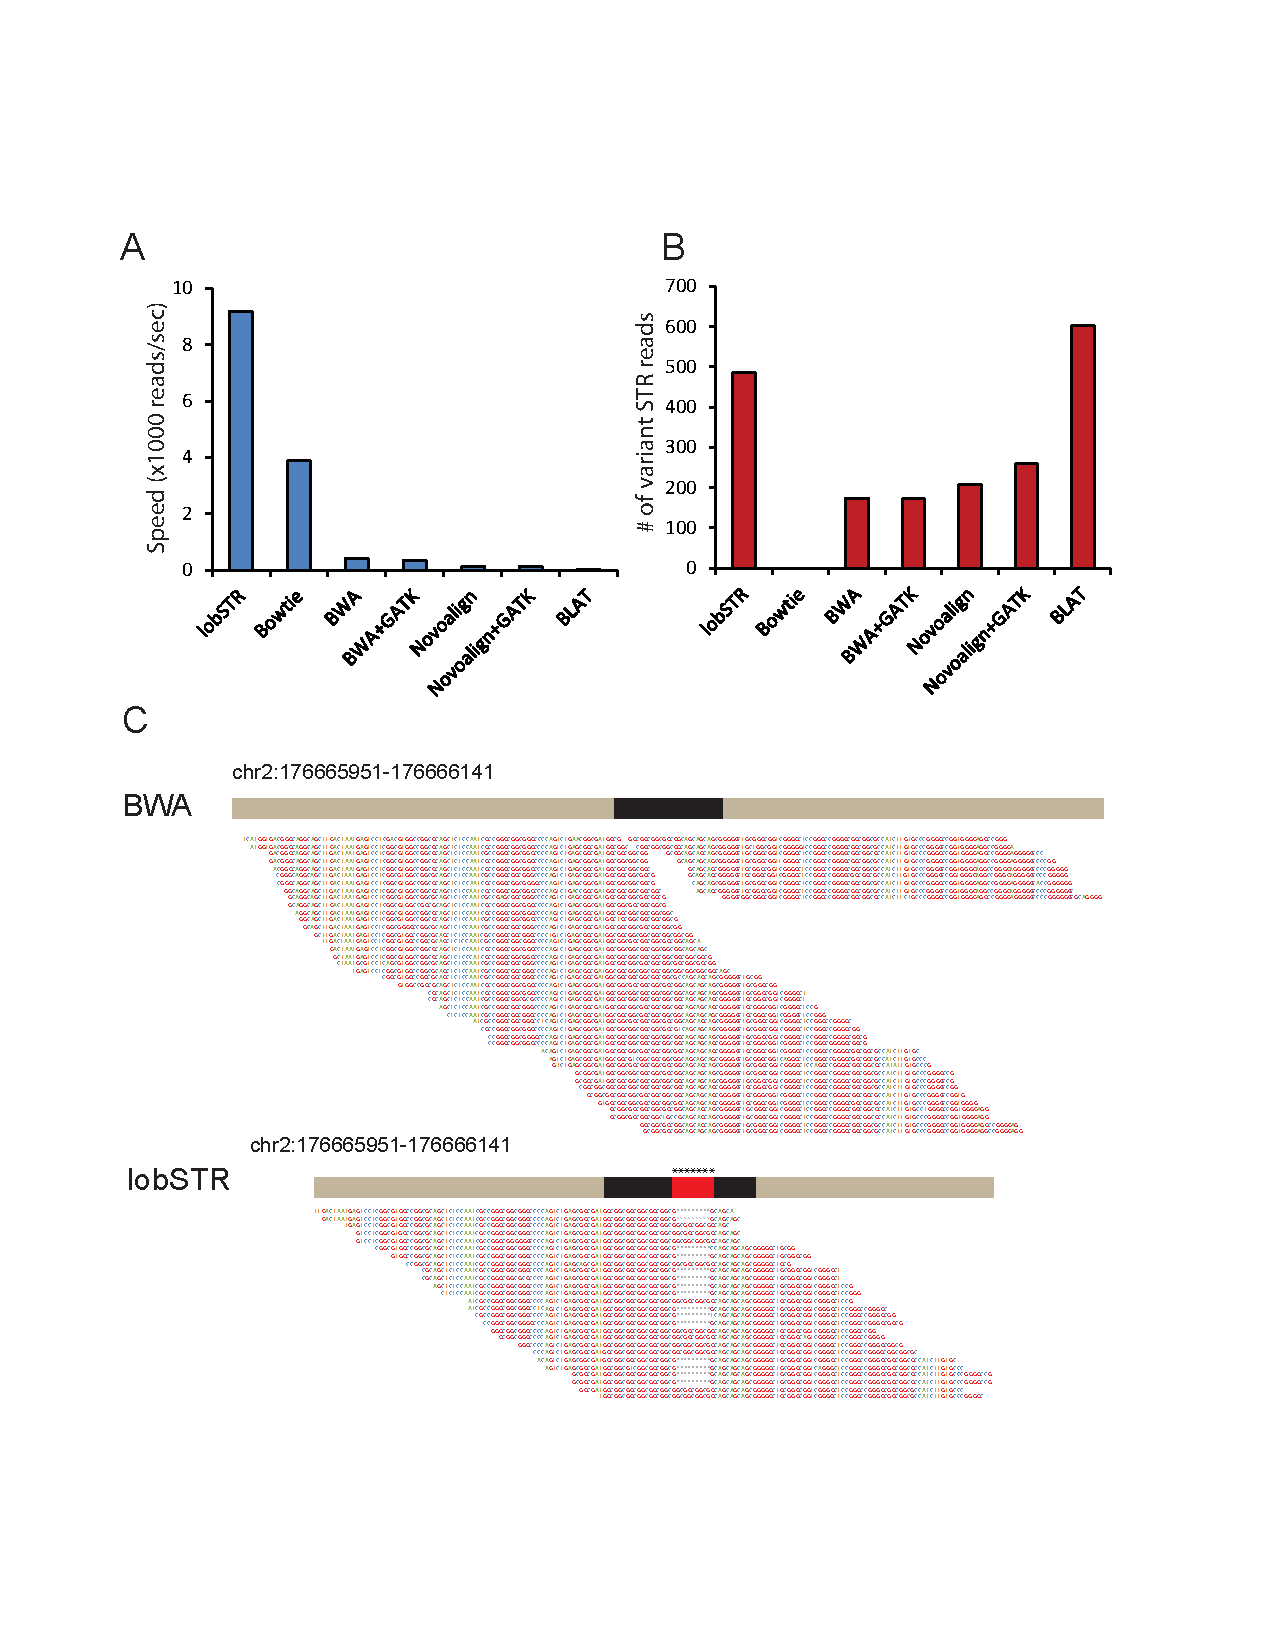
\includegraphics[width=0.5\textwidth]{Figures/Chapter2/Fig2.pdf}
\caption{\textbf{lobSTR shows an added value for STR profiling over mainstream techniques} \textbf{(A) Alignment speed (reads per second) of lobSTR, mainstream alignment and BLAT}. lobSTR processes reads between 2.5 and 1000 times faster than alternative methods \textbf{(B) The sensitivity of detecting STR variations of different alignment strategies.} Only BLAT detected more STR variations than lobSTR \textbf{(C) lobSTR accurately detects pathogenic trinucleotide expansions that are discarded by mainstream aligners.} The figure shows simulation results of the \emph{HOXD13} heterozygous locus with a normal and a pathogenic allele that contains 7 additional alanine insertions. BWA reports only the normal allele. Reads exhibiting a pathogenic STR expansion are not detected. lobSTR identifies both alleles present at the simulated locus. All positions are according to hg18.}
\end{figure}

Reporting STR reads with non-reference alleles is crucial for profiling pathogenic mutations. We further explored whether lobSTR can correctly detect disease alleles of dominant trinucleotide repeat expansion disorders. As test cases, we focused on two conditions that can be theoretically profiled using standard Illumina runs. The first condition was a GCN expansion in \emph{PABPN1} that causes oculopharyngeal muscular dystrophy (OPMD) \cite{BraisBouchardXieEtAl1998}, where the normal allele exhibits 10 repeats and the pathogenic allele spectrum for the dominant form is between 12 to 17 repeats \cite{PearsonNicholEdamuraCleary2005}. The second condition was a GCG expansion in \emph{HOXD13} that is implicated in synpolydactyly \cite{MuragakiMundlosUptonEtAl1996}, a severe limb malformation, where the normal allele is 15 repeats and the documented pathogenic allele spectrum is between 22-29 repeats \cite{PearsonNicholEdamuraCleary2005}. To simulate each condition, we generated 100 reads of length 101bp that were equally sampled from the disease locus consisting of a normal and pathogenic allele with 100bp flanking upstream and downstream regions with 1\% sequencing error rate. For both simulated disease conditions, lobSTR accurately aligned the normal and pathogenic reads to the correct location in the genome. All aligned reads were informative and the allelotyping step correctly assigned a heterozygous state to the disease loci with the correct repeat lengths: (10,15) for \emph{PABPN1} and (15, 22) for \emph{HOXD13}. In stark contrast, BWA failed to correctly align reads from the pathogenic alleles of both loci. Only reference reads were reported (\textbf{Figure \ref{fig:lobfig2}C}).

\subsection{Measuring lobSTR concordance using biological replicates}
To explore the precision of lobSTR, we conducted genome-wide STR profiling of blood and saliva samples from the same individual \cite{LamClarkChenEtAl2012}. These samples were sequenced using Illumina HiSeq2000 with 101bp PE to a mean autosomal coverage of 50x and 102x, respectively. lobSTR ran with default parameters on 20 CPUs and analyzed the two datasets within 12 and 22 hours respectively. After filtering loci with low quality calls, 143,793 shared STRs were covered in the two datasets with at least one read and 79,771 STRs were covered with 10 reads or more (\textbf{Figure \ref{fig:lobfig3}A}). 

We quantified the rate of discordant autosomal calls between the two samples. We focused on two measurements: the genotype discordance rate and the allelic discordance rate \cite{PompanonBoninBellemainEtAl2005}. The former reports as an error any mismatch between corresponding calls, whereas the latter reports only the fraction of discordant alleles in corresponding calls. For example, consider a locus that is called (A,B) in the saliva sample and (A,C) in the blood sample. This locus shows a single genotype discordance, but only 0.5 allelic discordance, since the A allele was correct. 

Both types of error greatly diminished with sufficient coverage (\textbf{Figure \ref{fig:lobfig3}B,C}). At 5x coverage, the genotype discordance rate was 11\% and the allelotype discordance was 5\%; At 21x coverage, the genotype discordance rate was 3\% and the allelotype discordance rate was 2\%. Similar to STR studies with capillary platforms \cite{WeberBroman2001}, most of the errors were generated in dinucleotide STR loci, whereas other types of STRs showed moderate and similar error rates. The dinucleotide error rates presumably stem from two factors: first, these loci usually show the highest heterozygosity rates \cite{ChakrabortyKimmelStiversEtAl1997,BrinkmannKlintscharNeuhuberEtAl1998,PembertonSandefurJakobssonEtAl2009}. Therefore, they require on average more sequence reads to be correctly called. Second, dinucleotide STRs are more prone to stutter noise \cite{Ellegren2004} and their higher error rates might be due to residual noise after lobSTR stutter deconvlution.

\begin{figure}[h!]
\centering
\label{fig:lobfig3}
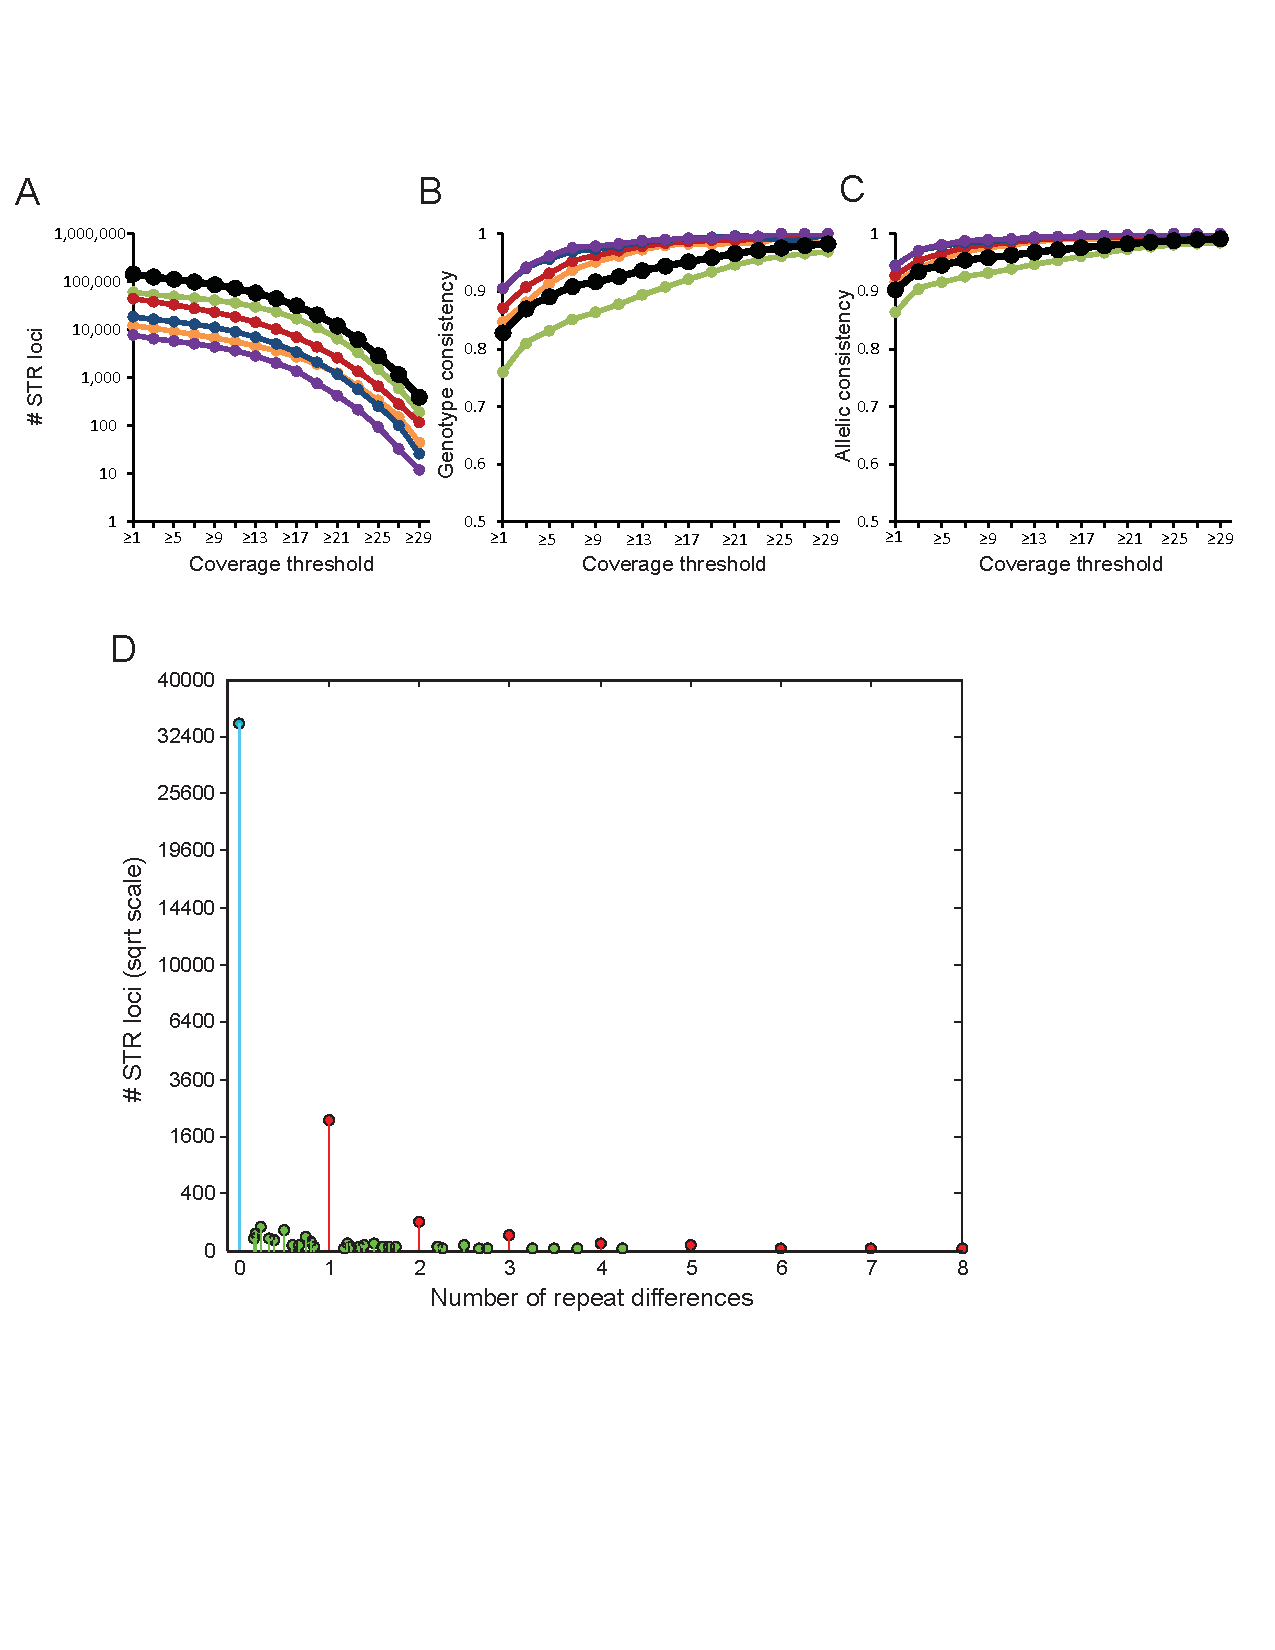
\includegraphics[width=0.5\textwidth]{Figures/Chapter2/Fig3.pdf}
\caption{\textbf{Measuring lobSTR consistency from two samples of the same individual} (A-C) (green - period 2, orange - period 3, red - period 4, blue - period 5, purple - period 6, black - all) \textbf{(A) Loci covered in both samples at increasing coverage thresholds.} \textbf{(B) The genotype discordance rate as a function of coverage threshold.} \textbf{(C) The allelic discordance rate as a function of coverage threshold.} \textbf{(D) Number of repeat differences at heterozygous loci.} Blue - no difference; red - integer numbers of repeat differences; green - non-integer numbers of repeat differences. Most discordance calls consist of a single repeat unit difference between calls in the two samples. Distance was measured as the second minimum distance between alleles of the two samples. The y-axis is given in a square root scale.}
\end{figure}

We further analyzed the STR length differences in discordant calls. To avoid analyzing errors that are simply due to allele drop-outs, we focused on discordant calls that were both heterozygous in blood and saliva. At a coverage of ≥5x, more than 90\% of the errors showed a single repeat unit difference and 99\% of the errors were within two repeat units (\textbf{Figure \ref{fig:lobfig3}D}). This indicates that incorrect alignment of STRs has a minimal effect on allelotyping results, and that stutter is likely the main source of noise. We also found that only 0.8\% of calls at heterozygous loci showed a difference due to an incomplete repeat unit. This highlights that lobSTR can determine STR alleles at a single base-pair resolution. 

\subsection{Tracing Mendelian inheritance using lobSTR}
To further explore lobSTR performance, we conducted a genome-wide STR profiling of a HapMap trio - a father (NA12877), mother (NA12878), and son (NA12882) -- from the CEU population that were sequenced using 100PE reads on a HiSeq2000 (\textbf{Table \ref{tab:lobtab2}}). The average autosomal coverage was 50x and average STR coverage was 14x. At $\geq$10x coverage threshold, 57\% of the STRs in the CEU trio had a non-reference allele. 

\begin{table}[h!]
\centering
\label{tab:lobtab2}
\begin{tabular}{l l l l l}
\hline
Individual	& Relationship & Input reads	& STR Aligned reads	& Mean STR Coverage \\
\hline
NA12878 &	Mother	& 1,708,169,546 &	3,398,933 &	14.8 \\
NA12877	& Father &	1,637,816,924	&3,212,073 &	14.1 \\
NA12882	& Son	& 1,625,404,856 &	3,183,795 &	14.0 \\
\hline
\end{tabular}
\caption{\textbf{Profiling STRs in Illumina reads from a HapMap trio.}}
\end{table}

In general, deviations of offspring's STR alleles from Mendelian inheritance (MI) indicate a potential calling error \cite{EwenBahloTreloarEtAl2000}. With 5x coverage across all trio members, the MI rate was 95\%; with 10x coverage, MI was 97\%; and with coverage threshold of 15 or more, MI was 99\%. (\textbf{Figure \ref{fig:lobfig4}A}). We also repeated the analysis only with discordant parental sites (for example, A/B call in one parent and A/C call in another parent). We noticed a drop to 93\% in the MI patterns with a low coverage threshold of 5x, which is mainly because of partial coverage of heterozygous sites in the parents. The MI rate was recovered to the same level with higher coverage threshold. At 17x coverage 99\% of sites showed a perfect Mendelian segregation pattern (\textbf{Figure \ref{fig:lobfig4}B}). 

\begin{figure}[h!]
\centering
\label{fig:lobfig4}
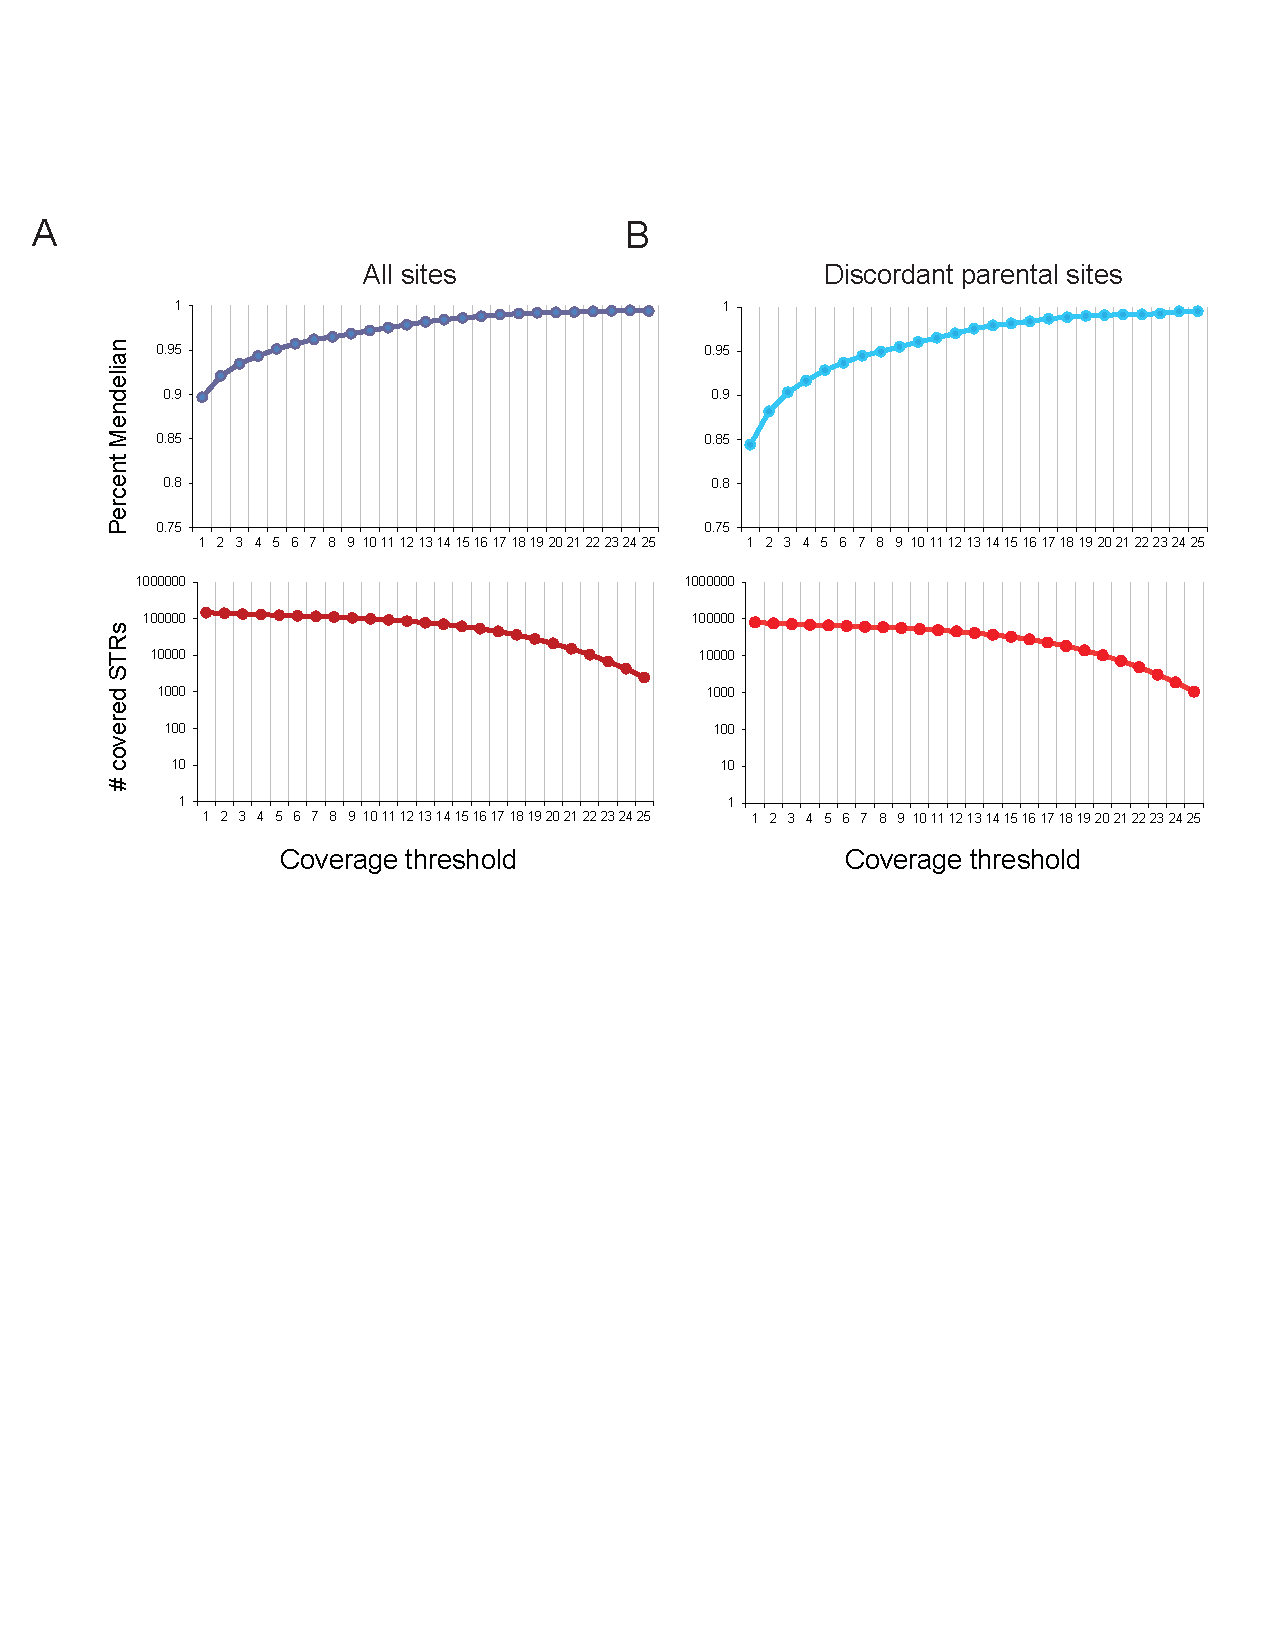
\includegraphics[width=0.5\textwidth]{Figures/Chapter2/Fig4.pdf}
\caption{\textbf{Validating lobSTR by Mendelian inheritance in a HapMap trio.} Mendelian inheritance (blue) rose to 99\% above 17x coverage. The number of covered loci at each coverage threshold is shown in red. \textbf{(A) Mendelian inheritance of all covered loci.} \textbf{(B) Mendelian inheritance of loci with discordant parental allelotypes.}}
\end{figure}

\subsection{Validating lobSTR accuracy with DNA electrophoresis}
We sought to compare lobSTR calls to the results of DNA electrophoresis, which is considered the gold standard for STR allelotyping. First, we focused on a set of STR markers that are used for forensic DNA fingerprinting. As an input for lobSTR, we sequenced a male genome from our lab collection with three runs of Illumina GAIIx for 101PE cycles that yielded ~740 million reads. The autosomal sequencing coverage was 36x according to alignment with mainstream algorithms. lobSTR identified 1.6 million informative reads that mapped to $\sim$140,000 STR loci, with an average of 4.91x coverage of diploid STR loci. In parallel, we used a commercial forensic kit to genotype 14 autosomal STR markers on a capillary electrophoresis platform. Thirteen out of 14 markers were covered by at least a single sequence read and 8 markers were covered by at least 3 sequence reads. The marker that was not covered spanned more than 129bp, exceeding the limit for detecting informative reads with the 101bp sequence reads.

We observed good concordance between lobSTR and the capillary results (\textbf{Table \ref{tab:lobtab3}}). lobSTR correctly called all but one of the 8 markers that were covered by at least 3 reads and most of the alleles in loci that were covered with 2 or less reads. Remarkably, some of these markers, such as D8S1179, displayed two heterozygous alleles that did not match the reference. Other alleles, such as in Penta D and Penta E, correctly returned 20bp and 25bp length differences from the reference allele, respectively. The capillary results of one tetranucleotide marker, THO1, exhibited a non-integer number of copies (9 repeats + 3bp). lobSTR reported exactly the same results, further demonstrating that STRs can be called within a single base pair resolution. lobSTR also correctly called a homozygous STR that was covered by a single read. In another 4 markers with coverage of ≤2x, lobSTR correctly called one allele and missed the other allele due to sequencing coverage. We observed only a single erroneous call due to stutter noise in the D5S818 locus. This homozygous locus was covered by three sequence reads: two correct and one with a single repeat expansion. With such a low sequencing coverage, the allelotyping algorithm was not able to identify the noisy read and assigned a heterozygous state to the locus. 

\begin{table}[h!]
\centering
\label{tab:lobtab3}
\begin{adjustbox}{width=1\textwidth}
\begin{tabular}{l l l l l l l l}
\hline
STR locus & lobSTR (bp) & Converted lobSTR & Capillary & Hg18 & Repeat & Coverage & Result$^a$\\
\hline
D8S1179 & -8/8 & 11/15 & 11/15 & 13 & [TCTA]n & 13 & Y\\
CSF1PO & -12/-4 & 10/12 & 10/12 & 13 & [AGAT]n & 13 & Y\\
TPOX & 0/12 & 8/11 & 8/11 & 8 & [AATG]n & 12 & Y \\
THO1 & 11/11 & 9.3/9.3 & 9.3 & 7 & [AATG]n & 11 & Y\\
D16S539 & 4/12 & 12/14 & 12/14 & 11 & [GATA]n & 5 & Y\\
D7S820 & -20/-8 & 8/11 & 8/11 & 13 & [GATA]n & 3 & Y\\
Penta D & -20/0 & 9/13 & 9/13 & 13 & [AAAGA]n & 3 & Y\\
D5S818 & 0/4 & 11/12 & 11 & 11 & [AGAT]n & 3 & E \\
D3S1358 & -4/-4 & 15/15 & 15/17 & 16 & [TCTN]n & 2 & P\\
PentaE & 25/25 & 10/10 & 10/15 & 5 & [AAAGA]n & 1 & P \\
FGA & -4/-4 & 21/21 & 21/24 & 22 & [TTTC]n & 1 & P\\
D18S51 & -12/-12 & 15/15 & 15 & 18 & [AGAA]n & 1 & Y\\
D13S317 & 4/4 & 12/12 & 11/12 & 11 & [TATC]n & 1 & P\\
\hline
\end{tabular}
\end{adjustbox}
\caption{\textbf{Capillary platform results versus lobSTR results for the CODIS set.} $^a$Y - both platforms agree. P - lobSTR reported only one allele out of two. E - lobSTR reported an allele that does not exist.}
\end{table}

Next, we evaluated lobSTR calls made in 12 low-pass sequenced genomes from the Human Genome Diversity Project (HGDP) \cite{GreenKrauseBriggsEtAl2010,ReichGreenKircherEtAl2010}. Five genomes had coverage of 1.4x-1.9x with 109bp reads, and the other seven had coverage of 4.8x-7.7x with 77bp reads (\textbf{Supplemental Table \ref{tab:lobsuptab3}}). One hundred and ninety five STRs with equivalent entries in the lobSTR reference have been genotyped in these genomes using DNA electrophoresis as part of the CEPH-HGDP panel \cite{RamachandranDeshpandeRosemanEtAl2005,PembertonSandefurJakobssonEtAl2009}. Combining lobSTR results from all datasets gave 59 comparable markers with coverage of 3-5 reads with a median coverage of 3x (\textbf{Supplemental Table \ref{tab:lobsuptab4}}). Despite the low coverage, lobSTR correctly returned 75\% of the genotypes and 85\% of the allele calls. Most of the alleles showed at least 5bp difference from the reference and some alleles showed a difference of 24bp and were correctly called. We did not observe a significant correlation between errors and the size of the variation. 

\subsection{Genome-wide STR profiling confirms previously locus-centric observations}
Encouraged by the accuracy and speed of lobSTR, we harnessed our pipeline to establish a reliable reference for future studies. Our input dataset was a male individual that, as of today, has been sequenced to highest coverage of 126-fold from a blood sample \cite{AjayParkerAbaanEtAl2011}. Fourteen billion sequencing reads were obtained from 100bp PE runs on Illumina GAIIx and HiSeq 2000. lobSTR ran for 26 hours using 25 CPUs. It aligned $\sim$6 million reads to approximately 180,000 STR loci out of the 249,000 in the Tandem Repeat Table reference with average coverage 20.82 for autosomal loci. The average reference allele length of undetected loci was 150bp, whereas the mean reference length of detected loci was 41bp. Therefore, in most cases, the undetected loci could not physically be spanned by a single read of the current sequencing length.

We assigned each autosomal STR to one of four allelotype categories: both alleles match the reference (homozygous reference), one allele matches the reference (heterozygous reference), both alleles do not match the reference but are the same (homozygous non-reference), and both alleles are different and do not match the reference (heterozygous non-reference). In all previous experiments, a coverage threshold of 20x resulted with near-perfect STR calling even for dinucleotide loci. To increase the reliability of our results, we focus the analysis on the 97,844 loci that were called with at least this sequencing coverage. The length distribution of these alleles in the reference was mainly between 25-50bp with a low number of very long STRs (\textbf{Figure \ref{fig:lobfig5}A}). 

Similar to the other genomes in this study, 55\% (52,338) of the STR loci differed from the reference: 22,271 (23\%) loci were heterozygous reference, 15,515 (16\%) loci were homozygous non-reference, and 14,552 (15\%) loci were heterozygous non-reference. The other 43,335 (45\%) loci were homozygous reference. Some of the variations reached to 49bp difference from the reference allele. On average, STR variations showed 6.3bp difference from the reference allele and 41\% of the variations were more than 5bp away from the reference (\textbf{Figure \ref{fig:lobfig5}B}). Thus, mainstream-dependent analysis pipelines that can tolerate only a few nucleotide indels, such as BWA, are likely to miss most STR variations.

The genome-wide STR dynamics reported by lobSTR confirm previous findings of locus-centric studies. The rate of STR polymorphism showed a striking correlation with the repeat unit length (\textbf{Figure \ref{fig:lobfig5}C}). Dinucleotide STRs are nearly equally likely to fall into any of the above four categories, whereas hexanucleotide STRs are most likely to match the reference. This trend matches results of a previous study that measured the mutation rate of a few hundreds of Y-STR loci as a function of repeat unit length \cite{JarveZhivotovskyRootsiEtAl2009}.  Similar to our results, the authors showed that penta- and hexanucleotide repeats mutate at half the rate of tri- and tetra-nucleotide repeats. We also found that the rate of STR polymorphism is significantly correlated to the length of the STR allele in the reference (\textbf{Figure \ref{fig:lobfig5}D}). The non-reference loci (n=52,338) had significantly greater lengths than loci that are homozygous reference (n=43,335) (p<0.05, one-sided Mann-Whitney test for each allelotype category versus reference) as previously reported in studies that analyzed a few dozen STRs \cite{BrinkmannKlintscharNeuhuberEtAl1998,Ellegren2000}. 

\begin{figure}[h!]
\centering
\label{fig:lobfig5}
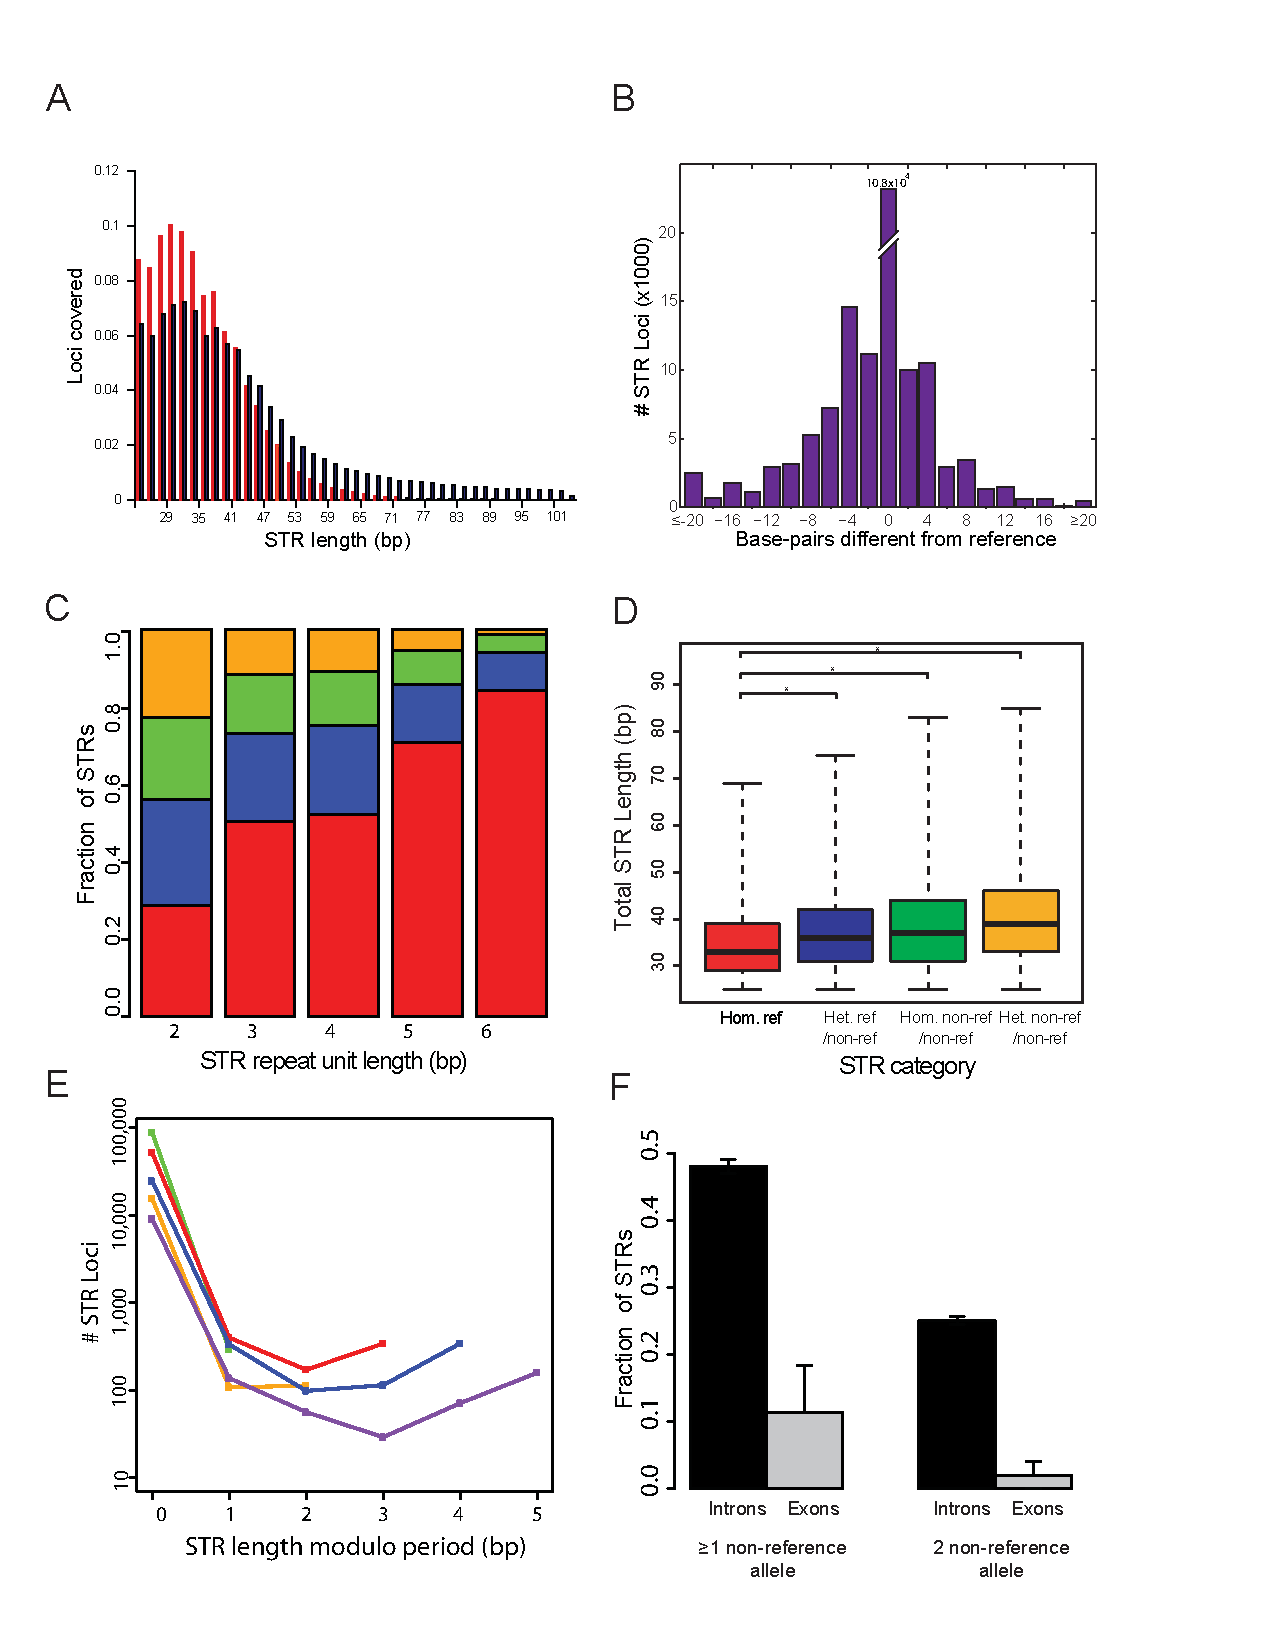
\includegraphics[width=0.5\textwidth]{Figures/Chapter2/Fig5.pdf}
\caption{\textbf{Genome-wide STR profile of an individual.} \textbf{(A) Distribution of STRs with 20x coverage or more as a function of the allele size in hg18.} \textbf{(B) Distribution of allele size differences from reference in lobSTR calls.} The average difference was 6.3bp away from the reference. \textbf{(C) STR polymorphism as function of period.} The number of STR alleles matching the reference sequence increases with increasing repeat unit length (the colors in the entire panel are as follows: red - homozygous reference, blue - heterozygous non-reference/reference, green - homozygous non-reference/non-reference, orange - heterozygous non-reference/non-reference \textbf{(D) Longer STR regions are more polymorphic.} The median STR length (thick black line) increases with the number of variant alleles. * denotes a significant (p<0.05) difference according to a one-sided Mann–Whitney test. Boxes denote the interquartile range and whiskers denote 3 times the interquartile range. \textbf{(E) lobSTR shows mutational trends at single base pair resolution.} The number of base pairs difference from reference modulo the period size versus the number of alleles detected (in logarithmic scale) is shown for each period (green - period 2, orange - period 3, red - period 4, blue - period 5, purple - period 6). Incomplete STR unit differences tend to differ by a full unit +/- 1bp from the reference. \textbf{(F) Fraction of trinucleotide STRs with non-reference alleles in introns versus exons.} 95\% confidence intervals are given by the error bars.}
\end{figure}

We also used lobSTR to determine genome-wide trends of STRs at single base pair resolution (\textbf{Figure \ref{fig:lobfig5}E}). Overall, 99\% of alleles varying from the reference allele showed differences that were complete multiples of the STR unit. This trend varied by period, with dinucleotide STRs least likely (0.3\%) to differ by an incomplete motif unit and hexanucleotide most likely (4.7\%).

Finally, lobSTR reported significant differences between repeat variations in intronic and exonic regions (\textbf{Figure \ref{fig:lobfig5}F}). Intronic trinucleotide STRs were twice as likely to exhibit at least one non-reference allele than exonic regions (0.480-0.502 95\% CI and 0.179-0.336 95\% CI for introns and exons, respectively), and nearly five times as likely to exhibit two non-reference alleles (0.107-0.119 95\% CI and 0-0.047 95\% CI for introns and exons, respectively). Significantly, lobSTR reported that 1.9\% (62 out of 3276) of the intronic trinucleotide STRs showed length differences that were not a multiple of three nucleotides. On the other hand, all reported exonic trinucleotide variants retained the reading frame. In addition, lobSTR allelotyped 34,667 intronic and 7 exonic non-trinucleotide STRs. Of the intronic non-trinucleotide STRs, 18,277 (53\%) showed at least one allele with a frameshift deviation, and 8,686 (25\%) showed two frameshifted alleles. Surprisingly, 3 of the 7 exonic loci, all tetranucleotides, showed expansions by units of 4bp, which would result in a frameshift mutation. In one case, in exon 8 of DCHS2, the frameshift variation was homozygous. This call was supported by 33 independent reads, showing a potential loss of function in this gene.

Taken together, the overall findings of lobSTR in this genome serve as a biological validation for the accuracy and utility of genome-wide STR profiling using our technique.

\section{Discussion}
STR profiling techniques have changed very little in the past two decades, relying on the faithful yet cumbersome capillary electrophoresis technique to scan a few dozen loci at a time. The advent of HTS has ushered in the opportunity to conduct genome-wide STR variation analyses. Here, we presented an end-to-end solution for this task. Our solution bypasses the gapped alignment problem, has no inherent indel limitation, and can reliably profile highly polymorphic STRs at a single base pair resolution. We provided a detailed comparison between lobSTR and popular mainstream aligners and showed that even with long reads, these aligners are significantly biased towards the detection of the reference allele. We have established the feasibility of lobSTR to profile STR loci from a total of 20 genomic datasets and demonstrated the strategy's accuracy by analyzing its consistency, ability to trace Mendelian inheritance, and comparing its results to orthogonal molecular techniques. Moreover, our genome-wide STR analysis confirms previous biological observations, which further highlights the algorithmic validity. 

lobSTR results from the trio genomes and the Ajay et al. genome consistently showed genome-wide polymorphism rates of 55\%-57\% for STRs with lengths 25bp and over. A recent study by McIver et al. \cite{McIverFondonSkinnerEtAl2011} evaluated the performance of STR calling using post-BWA alignment files with a set of quality rules. Using a mixture of Illumina 45-100bp reads and 454 reads from two trios in the 1000Genoems project, they reported that 1.1\% of the STRs with lengths of 20bp and over were polymorphic. We wondered if the polymorphism discrepancy between the studies could be explained by the shorter reading lengths in the McIver study that biased their calls to very short, less polymorphic STRs. However, when we ran lobSTR on the 1000Genomes CEU trio datasets (Methods), we found again that 57\% of the STRs were polymorphic (25,885 out of 45,461 STRs that were called with ≥5x coverage at the three genomes). These results suggest that STR profiling that is restricted by the default BWA indel tolerance -- 5bp for the Illumina datasets in the McIver et al. study -- can significantly reduce the sensitivity for observing STR variations. 

We envision that lobSTR will be used in parallel to conventional analysis pipelines in order to augment variation calling to STR loci. The fast running time of our algorithm should not impose a significant computational burden on users. A low coverage genome of 5x takes about an hour on a standard server with 25 CPUs, a high coverage genome of 30x takes eight hours using the same settings, and a ultra-high covered genome of 126x takes 26 hours (\textbf{Supplemental Table \ref{tab:lobsuptab2}}).

Currently, the major barrier for STR profiling is the sequencing read length, as the number of detectable STRs is limited to those that are entirely spanned by a single read. To test the effect of genomic coverage on STR profiling, we sampled reads from the 126x genome and calculated the amount of reported STRs (\textbf{Supplemental Figure \ref{fig:lobsup6}}). With genome-wide coverage of 40x, there are more than 100,000 STRs that will be pass an STR-coverage threshold of 10x. However, higher genomic coverage does not linearly improve the number of STRs that pass this threshold, marking a potential upper bound of sequencing read lengths of 100bp. We also explored the utility of the longer reads by Sanger, 454, and IonTorrent for STR profiling of personal genomes using lobSTR (\textbf{Supplemental Table \ref{tab:lobsuptab5}} and \textbf{Supplemental Text \ref{sec:lobsupptext}}). Longer reads indeed increased the number of reported STR loci compared to the same autosomal coverage by Illumina. However, out of these, Sanger seemed to be the only method to produce reliable STR reads. We expect that as sequencing reads continue to increase in both length and quality, lobSTR's performance will further improve and allow inclusion of a larger number of STR variations. Ultimately, these will include large pathogenic expansion, such as those in Huntington's disease, which can span more than 100bp. 

As of today, sequence analysis algorithms can detect almost any type of genetic variations, from SNPs \cite{GoyaSunMorinEtAl2010} and indels \cite{KoboldtChenWylieEtAl2009,GoyaSunMorinEtAl2010} to CNVs and chromosomal translocations \cite{ChenWallisMcLellanEtAl2009}. lobSTR adds a new layer of information with tens of thousands of highly polymorphic genetic variations that have a multitude of applications, from personal genomics, to population studies, forensics analysis, and cancer genome profiling.

\section{Methods}
\label{sec:lobmethods}
\subsection{Comparing lobSTR to mainstream aligners}
All alignment strategies were tested in a Linux environment, on a server with 4 twelve-core AMD Opteron 6100 and 128Gbyte of RAM. The following software versions were tested: BWA version 0.5.7, Bowtie version 0.12.7, and Novoalign freeware version 2.7.13, BLAT version 34, and GATK version 1.3-21.

The input was 5 million Illumina reads of the male sample from our lab collection. BLAT results were filtered to include only the top hit for each read. We suppressed multi-mappers in all other tools. Informative STR reads were identified by the intersectBed tool of the Bedtools packages \cite{QuinlanHall2010}. We converted CIGAR scores to the number of base pairs difference from the reference allele by counting any insertions or deletions falling within and directly adjacent to the STR region. Simulating reads from pathogenic STR loci was conducted using a simple Python script available by request from the authors. 

\subsection{Determining the expected number of non-reference reads}

A previous study by The Utah Marker Development Group has shown that 70\% of thousands of randomly chosen tetranucleotide STR loci are polymorphic. We also re-analyzed Payseur et al. data to infer the polymorphism rate in STRs with length ≥25bp in the assembled genome of Craig Venter using results reported in their Supplementary Tables 1-5. Concordant with the Utah study, this rate was 66\%.

The rate of non-reference STR reads is bounded between two extreme cases. The lower bound is that all polymorphic STRs are heterozygous with a reference allele. Thus, only half of the reads from variable loci will show a non-reference allele, which gives 33\% as a lower bound. The upper bound is that all polymorphic STRs are different from the reference in their two alleles. In this case, every read from a variable locus will show a non-reference allele, which gives 66\% as an upper bound.  

\subsection{Biological replicates analysis}
Raw reads for blood-derived and saliva-derived genomic DNA from the same individual were downloaded from the NCBI short read archive (\url{www.ncbi.nlm.nih.gov/sra}) with accessions SRX097307 and SRX097312, respectively. Loci in which (1) less than 75\% of reads agreed with the allelotype call in both samples or (2) the locus was covered in either sample by more than three times the mean coverage level were removed from the analysis.

\subsection{CEU trio data for Mendelian inheritance}
The HapMap CEU trio were NA12877 (father), NA12878 (mother), and NA12882 (son). Raw reads were downloaded from the European short read archive (\url{www.ebi.ac.uk/ena/}) with accessions ERP001228, ERP001229, and ERP001230, respectively. To determine if an STR followed Mendelian inheritance, we required that the alleles detected in the son could be explained by inheriting one allele from each parent. Low quality loci were filtered as described in Biological replicates analysis.

\subsection{Validating lobSTR accuracy using capillary electrophoresis}
Four Catch-All buccal swabs (Epicenter, QEC89100) were used to collect the DNA sample according to the manufacturer protocol. gDNA was extracted by QuickExtract (Epicentre), followed by phenol-chloroform purification and ethanol precipitation. Library preparation was performed according to the standard Illumina protocol. Three runs of 101bp paired-end with a GAIIx platform were used for sequencing. The study was approved by MIT's Committee on the Use of Humans as Experimental Subjects (COUHES). The general sequencing coverage was analyzed as previously reported \cite{ErlichEdvardsonHodgesEtAl2011}. 

Capillary electrophoresis results were obtained from Sorenson Genomics laboratory using the commercial Promega PowerPlex 16 system. To find the genomic positions of these loci, we downloaded corresponding primers that target these loci from the Short Tandem Repeats Internet Database (STRBASE) website (\url{http://www.cstl.nist.gov/strbase/}) of the US National Institute of Standards and Technology (NIST) and used the In Silico PCR tool on the UCSC genome browser to reveal their location. Two loci had proprietary primers and their genomic location could not be identified. The STR repeats in the sequencing file were converted to the PowerPlex allele nomenclature using the NIST definitions.

\subsection{Obtaining CEPH-HGDP STR allelotypes}
STR allelotypes along with a table of RefSeq reference alleles were downloaded from the Rosenberg lab site (\url{www.stanford.edu/group/rosenberglab/repeatsDownload.html}). The allelotypes were given as the number of repeats converted from PCR product size as described in Pemberton et al. \cite{PembertonSandefurJakobssonEtAl2009}. The repeat number is given as reference repeat number plus the difference in product size from the reference divided by the motif size. Sequence data were downloaded from the NCBI Short Read Archive with accessions: ERX004003, ERX004002, ERX004001, ERX004000, ERX0039999, ERX004007, ERX007978, ERX007977, ERX007976, ERX007975, ERX007974, ERX007973, ERX007972.

Using the STS marker table available from the UCSC Genome Browser, we converted the Pemberton et al. markers to hg18 genomic coordinates and annotated them using the TRF table. lobSTR calls that are supported by three or more reads were converted to the Pemberton results. Non-integer repeats reported by lobSTR were rounded to the smallest integer for compatibility with Pemberton data. Markers that could not be faithfully annotated were removed from the analysis.

\subsection{Genome-wide STR profiling of a deeply sequenced personal genome}
Raw sequencing reads for accession number ERP000765 were downloaded from the European Nucleotide Archive's Sequence Read Archive (\url{http://www.ebi.ac.uk/ena/}). The Mann-Whitney test was performed using the wilcox.test function in R. Confidence intervals were calculated using a normal approximation to the Poisson distribution, with a 95\% confidence interval of $\lambda\pm 1.96\sqrt{\lambda}$, where $\lambda$ is the estimated mean of the distribution. Only loci with greater than 20-fold coverage were included in the analysis. Exon and intron coordinates were obtained from the UCSC table browser for human genome build hg18. 

\subsection{1000 Genomes data analysis for the McIver Study}
The HapMap CEU trio were NA12878 (daughter), NA12891 (father), and NA12892 (mother). Raw sequencing reads for the CEU HapMap trios with length of at least 47bp were downloaded from the 1000 genomes NCBI ftp site (\url{ftp://ftp-trace.ncbi.nih.gov/1000genomes/ftp/}). 228, 274, and 214 files were included for individuals NA12878, NA12891, and NA12892. To accommodate the shorter read lengths, lobSTR was run with non-default parameters –fft-window-size 20 –fft-window-step 10, --maxflank 100, and –extend-flank 5. 

\section{Acknowledgements}
Y.E is an Andria and Paul Heafy Family Fellow. This publication was supported by the National Defense Science and Engineering Graduate Fellowship (M.G.) and by a fellowship from the Edmond J. Safra Bioinformatics program at Tel-Aviv University (D.G.). D.G. and S.R. acknowledge support from Israeli Science Foundation grant ISF 1227/09 and an IBM Open Collaborative Research grant. We thank Mona Sheikh, Dina Esposito, and Alon Goren for useful comments on the manuscript, Assaf Gordon for his assistance with multithreading programming, Cole Trapnell for his assistance with preparing lobSTR executables, Mona Sheikh and Sam Sinai for testing lobSTR code, and Dina Esposito for preparing samples for genotyping. 

\section{Supplemental Text}
\label{sec:lobsupptext}
\subsection{lobSTR algorithm}

\subsubsection{Sensing}
The aim of the sensing step is to find informative reads and characterize their STR sequence. The first task of the algorithm is to detect whether a read contains a repetitive sequence. The algorithm breaks the sequence read into overlapping windows with length of $w$ nucleotides and $r$ nucleotide overlap between consecutive windows. In practice, we use $w=24$ and $r=12$. Then, it measures the sequence entropy of each window, according to:

\begin{equation}
E(S_j) = -\sum_{i \in \Sigma}f_i \log_2 f_i
\end{equation}

where $E$ is the entropy, $S_j$ is the sequence of the $j$-th window, $\Sigma$ is the alphabet set, $i$ is a symbol in the alphabet, and $f_i$ is the frequency of symbol $i$. A fully random sequence results in the maximal entropy score that equals to $\log_2(|\Sigma|)$, whereas a repetitive sequence overuses a few symbols and results in a low entropy score, ideally zero in the case of a perfect homopolymer run.

The entropy score proved extremely powerful in discriminating STR sequences from other genomic sequences (\textbf{Supplemental Figure \ref{fig:lobsup2}A}). We calculated the entropy score of sliding windows of 24bp from all documented human STR sequences of repeat unit length of 2-6bp that span up to 100bp. In parallel we scored one million randomly sampled human genomic sequences of 24bp. Then, we classified the input sequences according to their entropy score. The area under the receiver-operating curve (ROC) was 98.3\% when the entropy measurement used the four nucleotides as the input alphabet. We further boosted the classification performance by calculating the entropy using dinucleotide symbols, meaning that “AA” maps to one symbol, “AC” maps to a different symbol, and so forth. In this case, the area under the ROC climbed to 99.4\%, which renders it a nearly perfect classifier. Accordingly, lobSTR uses the dinucleotide symbols for the entropy measure, and we empirically found that an entropy threshold of 2.2 bits provides the optimal performance in terms of speed and number of aligned STR reads.

lobSTR uses the pattern of entropy scores to identify informative reads that fully encompass STR regions. These reads display a series of windows with entropy score below-threshold (the STR region) that are flanked by one or more windows with entropy score above-threshold (the non-repetitive regions) (\textbf{Supplemental Figure \ref{fig:lobsup2}B}). The algorithm only retains reads that follow this pattern. Approximately 97\% of whole genome sequence reads are excluded by this rapid procedure. This significantly contributes to the algorithm's speed, since only a few simple entropy calculations are required to identify the informative STR reads in massive sequencing datasets.

The next task of the sensing step is to determine the length of the repeat unit. Most STR loci do not contain a perfect series of the same repeat unit \cite{Benson1999}. We took a spectral analysis approach that quickly integrates information over the entire STR region to reliably identify the repeat consensus even in imperfect repeats \cite{SharmaIssacRaghavaEtAl2004}. Starting from the window with the lowest entropy score, consecutive windows scoring below the threshold are merged. The sequence of the merged repetitive region is represented as $M$, an $n \times 4$ binary matrix, where $n$ is the number of nucleotides in the repetitive region, the $i$-th row of the matrix corresponds to the $i$-th position of the sequence, and each column corresponds to a different nucleotide type (A,C,G,T). For instance, the DNA sequence ACCGT is represented as:

\begin{equation}
\left[
\begin{array}{c c c c}
1 & 0 & 0 & 0 \\
0 & 1 & 0 & 0 \\
0 & 1 & 0 & 0 \\
0 & 0 & 1 & 0 \\
0 & 0 & 0 & 1 \\
\end{array}
\right]
\end{equation}

The power spectrum of the STR matrix is calculated by performing a Fast Fourier Transform along the columns of the matrix:

\begin{equation}
S(f) = \sum_{y=1}^4 \left( \sum_{x=1}^n M_{x,y} \cdot e^{-\frac{2\pi ixf}{n}} \right) ^2
\end{equation}

Where $M_{x,y}$ is the element in the $x$-th row and $y$-th column of $M$.

STRs have a unique fingerprint in the frequency domain \cite{SharmaIssacRaghavaEtAl2004,ZhouDuYan2009}. Similar to repetitive signals in the time domain, the spectral response of STR elements is characterized by harmonics - a strong signal in recurrent frequency bins and a weak signal in other bins (\textbf{Supplemental Figure \ref{fig:lobsup2}C}). The peaks of the harmonics for a repeat unit of length $k$ dwell in the $\frac{ni}{k} \text{ mod } n$ bins, $i = \{ 0, \pm 1, \pm 2, \hdots \}$. For instance, in a case of n=24, a dinucleotide STR generates a strong signal in bins 0 and $\pm$12. A trinucleotide STR generates a strong signal in bins 0, $\pm$8, and $\pm$16. The algorithm integrates over the normalized energy of the first harmony (i.e. $i$=1) of each possible repeat unit between 2 to 6bp. The consensus repeat unit length is selected according to the highest energy of the corresponding frequency bin (\textbf{Supplemental Figure \ref{fig:lobsup2}D}). Some STR regions may show strong signals in more than one energy bin (i.e., repeats of period 4 show strong energy in both the second and fourth harmonics, and repeats with several insertions or deletions may have more than one strong harmonic). If the second highest harmonic has energy within 30\% of the highest, lobSTR will attempt alignment using the second best period choice if alignment using the first choice fails.

Finally, the algorithm determines the actual STR sequence. It uses a rolling hash function to record all possible $k$-mers in the STR region, where $k$ is the reported repeat unit length described above. The most frequently occurring $k$-mer is set to be the repeat unit of the STR. The output of the sensing step is (a) the consensus sequence of the STR's repeat unit in the canonical form (see Supplemental Methods for the canonical form definition) (b) the sequence read divided into three regions: the STR region, and upstream and downstream flanking regions that correspond to the location of the above threshold windows. 

\subsubsection{Alignment}
The aim of the alignment step is to reveal the identity and the repeat length of an STR-containing read. We do not attempt to align the entire sequence read to the genome to avoid time-prohibitive gapped alignment. Instead, lobSTR employs a divide-and-conquer approach. It separately anchors the upstream and downstream flanking regions of STR-containing sequence reads, without mapping the STR region itself. This procedure identifies the genomic location of the STR and reveals the repeat length by measuring the distance between the flanking regions.

A major challenge of the divide-and-conquer approach is to specifically map the short flanking regions to the genome. To circumvent this problem, we restrict the alignment to STR loci with the same repeat sequence that was reported by the sensing step. We built a reference that holds the flanking regions of all the 240,351 STR loci with repeat unit 2-6bp in the human genome according to the Tandem Repeat Finder table \cite{Benson1999}. The flanking strings are compressed using a Burrows Wheeler Transform \cite{BurrowsWheeler1994} (BWT) to allow efficient searching. All flanking strings of STRs with the same repeat structure are organized under the same BWT structure (Supplemental Methods). Thus, lobSTR only searches a single BWT data structure that corresponds to the repeat sequence, which typically holds up to a few thousand loci. Then, lobSTR intersects the potential mapping positions of the upstream and downstream regions to identify a single compatible location and excludes multiple mappers. This procedure not only speeds up the alignment, but enables higher rates of unique mapping even when the flanking regions are only a few nucleotides long. 

To determine the length of the STR in the read, the algorithm uses the following equation: 

\begin{equation} \label{eq:alnstep}
L = s - (d - u ) + L_{ref}                                                                  
\end{equation}

Where $L$ is the observed STR length, $s$ is the length of the sequence read, $d$ is the genomic coordinate of the last nucleotide in the downstream region, $u$ is the genomic coordinate of the first nucleotide of the upstream region, and $L_{ref}$ is the length of the STR region in the reference genome. 

One important aspect of Eq. 4 is that inaccuracies in the sensing step regarding the exact boundaries of the STR do not affect the reported length of the STR. However, insertions or deletions in the flanking regions might be reported as STR differences, although they are not actual differences in the STR region itself. To mitigate this issue, lobSTR performs local realignment of the entire read once a match is found using the \cite{NeedlemanWunsch1970}. Indels that are detected in the flanking regions are not taken into account and removed from Eq. \ref{eq:alnstep}, providing accurate length calling of the STR region. In addition, the local realignment is used to produce a CIGAR string with the locations of the indels in the read. Downstream genotype callers can use the output of lobSTR to call SNPs and indels in the STR region and its flanking regions. 

The output of the alignment step is the genomic coordinates of the aligned read, the strand, the STR region extracted from the read, the STR motif, the nucleotide length difference compared to the reference genome as described above, the CIGAR string, and the realignment score. We report the alignments in a custom tab-delimited format, as well as in the BAM format \cite{LiZhaoLinEtAl2009} to ensure compatibility with other downstream bioinformatics tools.

\subsubsection{Allelotyping}
The aim of the allelotyping step is to determine the most likely alleles of each STR locus by integrating information from all aligned reads and the expected stutter noise, which is created due to in vitro slippage events during sample preparation. This part of the program uses a BAM file as input and reports the allelotype calls.

By analyzing real sequencing data, we found that the length of the repeat unit is a major determinant of the stutter noise distribution (Supplemental Methods). In accordance with the mutation dynamics of STRs previously reported \cite{Ellegren2004}, short repeat units are associated with higher stutter noise and long repeat units are more immune to noise (\textbf{Supplemental Figure \ref{fig:lobsup3}A}). We did not find a significant association between stutter noise and the length of the STR (\textbf{Supplemental Figure \ref{fig:lobsup3}B}) as was observed in past studies \cite{HaugeLitt1993}.

We developed a generative model for stutter noise that consists of two steps: (a) with probability $\pi(k)$, the read is a product of stutter noise, where $k$ denotes the repeat unit length (b) if the read is a product of stutter noise, then with probability $\mu(s; \lambda_k)$, the noisy read deviates by $s$ base pairs from the original allele, where $\mu(s; \lambda_k)$ is a Poisson distribution with parameter $\lambda_k$. The probabilities that the deviation is positive (repeat expansion) or negative (repeat contraction) are equal. 

The user has two options to estimate the model parameters $\pi(k)$ and $\lambda_k$. In the case of a male genome, the user can instruct lobSTR to scan the hemizygous sex chromosomes to accumulate unambiguous data about stutter noise distribution. The algorithm observes the stutter probability for each repeat unit length and uses a logistic regression to infer $\pi(k)$ (\textbf{Supplemental Figure \ref{fig:lobsup3}A}) and a Poission regression to learn $\lambda_k$. In the case of a female genome, users can use pre-computed values either from our observations or analyze male data in their collection. 

Overall, the probability of generating a read with $L$ bp in the STR region from a hemizygous locus with an STR with A bp in the STR region is:

\begin{equation}
P(L|A, k) = 
\begin{array}{c c}
1-\pi(k) & \text{if } L=A \\
\frac{\pi{k}}{2} \mu(|A-L|-1, \lambda_k) & \text{otherwise} \\
\end{array}
\end{equation}

In a diploid STR locus with $A$ and $B$ repeat lengths, we use the following heuristic to approximate the likelihood of observing a read with length $L$:

\begin{equation}
P(L|A,B,k) = max(P(L|A,k),P(L|B,k))
\end{equation}

This heuristic was found to be more robust when the two STR alleles have large length differences.

Let $\vec{R}$ be a vector that describes the STR lengths of sequence reads from the same locus after removing PCR duplicates (Supplemental Methods). Since each remaining sequence read is a product of an independent series of PCR rounds, we assume that the stutter noise of different entries in $\vec{R}$ is independent. Accordingly: 

\begin{equation} \label{eq:lobloglik}
\log[P(\vec{R}|A,B,k) = \sum_{L\in \vec{R}}\log[P(L|A,B,k)]]
\end{equation}

Thus, the most likely allelotype call is when Eq. (7) is maximized with respect to $A$ and $B$. To find the best bi-allelic combination, we simply iterate over all possible pairs of STR lengths observed at the interrogated locus and compute the likelihood of generating the observed data given the noise model. For example, if $\vec{R}=(13,13,12,12,12)$, we calculate the log likelihood in Eq. \ref{eq:lobloglik} for the combinations: ($A$=12,$B$=12), ($A$=12,$B$=13), and ($A$=13,$B$=13). In addition to the log likelihood score, we require a minimum threshold of the variant allele in order to call a locus as heterozygous, with a default threshold of 20\% and a minimum percentage of reads supporting the resulting allelotype, which defaults to 50\%. In the case of sex chromosome loci for a male sample, only homozygous allelotypes are considered. The most likely $(A,B)$ combination is reported.

For each STR locus, the allelotyping step returns the chromosome, start, and end of the locus, the STR motif and period, the reference repeat number from TRF, the allelotype call given as the number of base pairs difference from reference for each allele, coverage, number of reads agreeing with the allelotype call, the number of reads disagreeing with the allelotype call, and the number of reads supporting each observed allele.

\subsection{Technical Evaluation of lobSTR}
\subsubsection{Comparison between lobSTR sensing step and the TRF tool}
Tandem Repeat Finder was developed to find repetitive elements in large sequence contigs. Conceptually, it could also process short reads and replace the lobSTR sensing step in characterizing STR repeats. To compare the performance of the two lobSTR sensing step and TRF, we challenged the two tools with a set of 5 million 101bp whole-genome Illumina reads. To make a fair comparison, TRF was restricted to a maximum repeat unit period of six nucleotides and lobSTR ran on a single CPU. 

Our results indicate that lobSTR's sensing step is significantly more adequate for high throughput sequencing data. lobSTR running time was just under 8 minutes compared to 6.5 hours for TRF (about 50 times slower, \textbf{Supplemental Figure \ref{fig:lobsup4}A}). This means that analyzing personal genomes would take weeks instead of half a day of running time. Moreover, 94\% percent of reads that were flagged as informative by both methods were reported with the same repeat sequence (\textbf{Supplemental Figure \ref{fig:lobsup4}B}). Most of the discordant results occurred in STRs of period 5 or 6 where lobSTR and TRF could not reach a consensus regarding the repeat unit of imperfect repeats. Last, lobSTR flagged as informative 75\%-85\% of the reads that were flagged by TRF, with higher sensitivity with increasing STR purity (\textbf{Supplemental Figure \ref{fig:lobsup4}C}). Thus, while lobSTR cannot detect every read that is detected by TRF, it does reach high sensitivity with 1/50 of the running time which is more suited to the ultra-exponential trajectory of high throughput sequencing datasets. 

\subsubsection{lobSTR performance with different sizes of STRs}
The size of the flanking regions determines the mappability of STR containing reads. In order to find the minimal flanking regions, we extracted genomic sequences of 100bp upstream and downstream of all STRs in the TRF table and organized them in prefix trees according to their canonical repeat unit. Then, we exhaustively aligned target STRs by allowing increased flanking region lengths and reporting the minimal length when a unique and correct alignment was achieved. Since this step is time prohibitive, we focused our analysis on a set of 2050 STR from the CODIS set, exonic regions, and genealogical Y-STR markers that were covered by 100bp reads. Our results show that a total of 8-9bp of upstream and downstream flanking regions is a lower bound for unique alignment of 80\% of tested STRs (\textbf{Supplemental Figure \ref{fig:lobsup5}A}). This means that with 100bp reads, lobSTR can theoretically detect STR regions of up to 84nt.  

We also determined the power of lobSTR to detect reads with very short STR regions due to strong repeat contraction. These reads have higher entropy and might not cross the threshold in the sensing step. To simulate this effect, we ran TRF on a set of 5 million input reads in a setting returning detected STRs as few as 12bp long. We then measured the performance of lobSTR to detect reads from these short STR loci and found that repetitive elements with 12nt were well captured (\textbf{Supplemental Figure \ref{fig:lobsup5}B}). Our overall results suggest that lobSTR can perform well in detecting STRs of 12-84bp. 

\subsubsection{lobSTR performance on various sequenecing platforms}
To test lobSTR performance on other sequencing platforms than Illumina, we ran the algorithm on publicly available genomes from three different platforms: Sanger (Craig Venter genome) \cite{LevySuttonNgEtAl2007}, 454 (Watson genome) \cite{WheelerSrinivasanEgholmEtAl2008}, and IonTorrent (Moore genome) \cite{RothbergHinzRearickEtAl2011}. In the absence of orthogonal information about STRs in these genomes, we estimated the performance of lobSTR by several parameters: (a) the ratio of aligned STR reads to the total input (b) the fraction of reads with a non-integer number of repeat units different from reference (c) the coverage of STR loci (\textbf{Supplemental Table \ref{tab:lobsuptab5}}).

As expected from its long read length and high accuracy, Sanger sequencing showed the best performance. It produced the best ratio of reads that aligned to STR loci and showed the lowest fraction (7.3\%) of STR reads with a non integer number of repeat units difference from reference. Importantly, the Sanger fraction of non-integer number of repeats was close to the Illumina fraction (8.0\%). 454 produced more STR aligned reads per amount of sequencing data than Illumina but 25\% of the STR reads showed a non-integer number of repeat units. IonTorrent showed the worst performance in both the ratio of STR reads and non-integer repeats.  The high number of STR reads with non-integer repeat units is presumably because 454 and Ion Torrent exhibit indel error when sequencing homopolymer runs that are abundant in many types of repeats (e.g. AAAAC).

Our results show that lobSTR can process sequencing files from other high throughput sequencing platforms and report STR reads. However, the accuracy of the STR calls is expected to be inferior to that reported for Illumina. We expect that improvement in homopolymer sequencing in 454 and Ion Torrent will make their datasets more amenable to STR profiling. 

\subsubsection{STR coverage as a function of input libraries}
We sought to explore the function of STR coverage by lobSTR to the genome-wide coverage of autosomal regions. Using the genome sequenced to 126x coverage by Ajay, et al. \cite{AjayParkerAbaanEtAl2011} described in the main text, we sampled from the BAM file produced by lobSTR for a range of desired coverage levels. We then allelotyped only this subset of reads and counted how many STR loci were covered by at least one informative read (\textbf{Supplemental Figure \ref{fig:lobsup6}}).

As a rule of thumb for 100bp reads, we found that STRs obtain an average coverage of approximately one-fifth the genome-wide autosomal coverage. In addition, we found that around 60,000 to 80,000 STRs can be covered by at least a single sequence read even with a shallow genomic coverage of less than 5x. The number of STRs covered by at least 1 read rapidly plateaued to ~180,000 loci after a genome-wide coverage of around 40x. 

Certain STR loci in the TRF table cannot be detected regardless of the coverage. The main limitation is that 100bp reads cannot span 16\% of the STR entries in TRF. Other STR regions dwell in repetitive elements and generate non unique alignments, such as the Y-STR marker DYS464a/b/c/d/e/f, which has multiple locations \cite{KehdyPena2010}. Reads from these loci will be flagged as multi-mappers and will be removed from the analysis. Finally, some STR regions do not pass the entropy threshold due to their imperfect repeat structure and will not be detected using lobSTR default parameters. This can be circumvented by lowering the lobSTR entropy threshold but will require substantial running time.

\subsubsection{Coverage bias in heterozygous loci}
We found a slight but statistically significant bias of 1:1.06 in the number of reads towards the shorter alleles in heterozygous loci (one sided Mann-Whitney test, p $<$ 0.05). For instance, there are on average $\sim$2 more reads that support the shorter allele when an STR is covered by 30 reads.  This observation can be explained by a PCR bias as reported by a previous study \cite{WattierEngelSaumitou-LapradeEtAl1998}. Since this small effect only becomes visible in ultra-high coverage STRs, lobSTR does not currently correct for it.

\subsubsection{Hardware requirements}
With the given TRF reference, lobSTR reaches a peak memory footprint of 0.3Gb regardless of input size and can process about 0.6 million reads per minute on a single processor. On 25 processors, lobSTR took 26 hours to process the genome sequenced to 126x coverage described in the main text, rendering the hardware requirements of lobSTR well within the range of routinely performed bioinformatics tasks such as SNP calling and short read alignment. The processing times for several genomes analyzed in this paper are given in \textbf{Supplemental Table \ref{tab:lobsuptab2}}. 

\section{Supplemental Methods}
\subsection{Building an STR reference}
The STR reference was built according to the entries of the Simple Tandem Repeat Table for human reference genome build hg18, available from the UCSC genome browser (this reference was used for all other results as well) \cite{Kent2002}. The table was filtered to include STRs with repeat unit lengths of 2-6bp. Nearly half of the loci are dinucleotide repeats. The number of STR loci with each repeat unit length is given in \textbf{Supplemental Table \ref{tab:lobsuptab6}}. The 10 most common repeat units are given in \textbf{Supplemental Table \ref{tab:lobsuptab7}}. The median length of STR regions is near 40bp for each repeat unit length. The distribution of repeat region sizes increases slightly with the repeat period, and less than 6\% of STR loci span more than 100bp (\textbf{Supplemental Figure \ref{fig:lobsup7}}). The majority of reference STRs lie in intergenic regions. 1,221 reference loci overlap exonic regions.

STRs display cyclic ambiguity. For example, consider the following STR: GACGACGACGACGAC. This STR can be described in three ways (GAC)5, (ACG)5, or (CGA)5, as well as by (GTC)5, (CGT)5, or (TCG)5 on the reverse strand. The sequence repeats in the TRF table are reported in a redundant format that does not distinguish between cyclic shifts. We converted all repeat sequences in the table to a canonical form in which the repeat sequence is the lexicographically highest among all possible cyclic representations of the sequence and their reverse complements. STRs whose repeat sequences contradicted the canonical repeat unit length, such as TTT listed as period 3 instead of 1, were removed from the reference. lobSTR reports the period of the STR according to the canonical form.

For mapping Illumina reads, the reference consists of the ±150bp flanking regions of each STR locus. We grouped reference sequences from loci with the same canonical STR repeat unit into a single FASTA file and built a single BWT index using the BWA function ``bwa index –a is'' on each file.

\subsection{PCR duplicate removal}
By default all reads with the same 5' coordinate and length are flagged as PCR duplicates and collapsed into a single read. The user has the option to turn PCR duplicate removal off. If a group of PCR duplicate reads are associated with more than one STR length, lobSTR uses a majority vote to determine the STR length of the collapsed read. If the majority vote results in a tie, the STR length of the collapsed read is determined according to the read with the highest average quality score. All reported sequencing coverage numbers are given after removing PCR duplicates.

\subsection{Building a model for stutter noise}
We analyzed Illumina reads from approximately 6,000 hemizygous loci on the sex chromosomes of a male individual from our lab collection. We assumed that the mode of the STR lengths in each locus was the true allele. All reads differing from the modal allele differed by either one (76\% of noisy reads) or two (24\% of noisy reads) repeats. Initial analysis of the stutter noise was done using R and was implemented in C++/R in the allelotyping script that is part of the lobSTR package.

\subsection{lobSTR implementation details}
lobSTR is written in C/C++ and calls on R for allelotyping step. We made an effort to use existing, highly optimized libraries for lobSTR implementation to increase the speed of the program. The spectral analysis in the detection step was implemented using FFTW \cite{FrigoJohnson1998} and the alignment step uses extensive parts of the BWA code \cite{LiDurbin2009a} for BWT-indexing and the BamTools library \cite{BarnettGarrisonQuinlanEtAl2011} for reading and writing BAM files. 

From the user's perspective, lobSTR consists of running two simple programs: one command for sensing and alignment, followed by a command for allelotyping aligned reads from a BAM file. In the simplest setting, the user just needs to specify the input files, the prefix name of the output files, and the location of the reference, which is provided with the software. However, we also provide advanced options that include modification of the detection threshold, re-sizing the FFT windows, and increasing the tolerance to sequencing errors in the flanking regions (\textbf{Supplemental Table \ref{tab:lobsuptab1}}). The user can also build a custom reference using a tool in the lobSTR package.

\subsection{lobSTR comparison across sequencing platforms}
Raw reads for the Watson genome were downloaded from the NCBI short read archive with accession SRX000114. Reads for the Moore genome were downloaded from the Europe	an short read archive with accession ERS024569. Reads for the Venter genome were downloaded from TraceDB (Genbank accession ABBA00000000). For the Venter genome, we trimmed the first 50bp of every read due to the high error rate at the beginning of Sanger sequence reads and discarded reads whose length after trimming was less than 100bp.

\pagebreak
\section{Supplemental Figures}

\subsection{Supplemental Figure 1}
\begin{figure}[h!]
\centering
\label{fig:lobsup1}
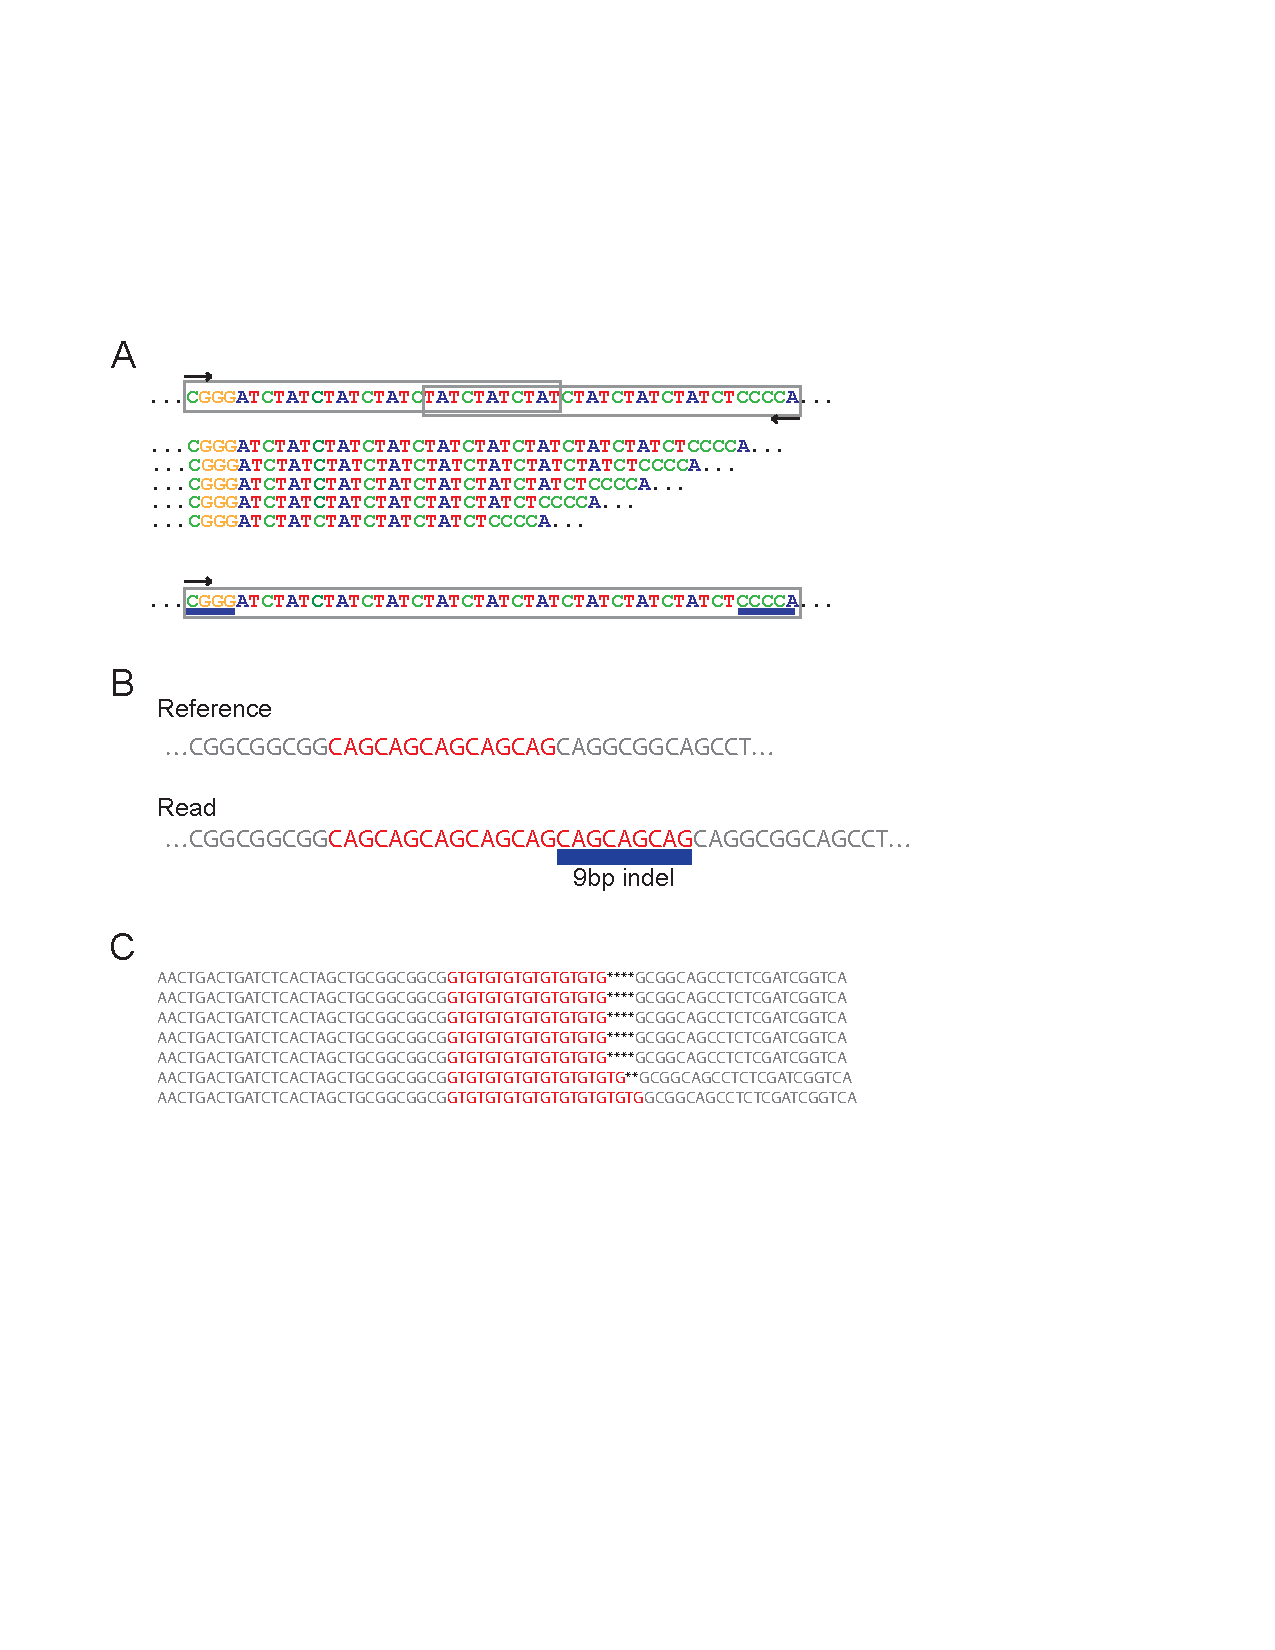
\includegraphics[width=0.65\textwidth]{Figures/Chapter2/SuppFig1.pdf}
\end{figure}
\textbf{Feasibility of STR profiling with HTS.} \textbf{(A) Long paired-end reads are not a sufficient condition for STR profiling.} Each read end (gray box) only partially covers the STR locus (top). Although the ends overlap and together span the entire locus, the number of repeat units is ambiguous (middle), since the exact overlap length is unknown. Single-ends that span the entire STR are informative (bottom). The single-end read (gray box) encompasses the flanking regions outside the STR locus (blue lines). These allow the read to be anchored to obtain unambiguous information about the STR length. \textbf{(B) Modest STR polymorphisms translate to large indels.} Thus, detecting non-reference STR reads requires cumbersome processing times by mainstream aligners \textbf{(C) An example of stutter noise due to PCR slippage events.} A series of sequence reads were obtained from the same allele. The last two reads have additional repeats due to PCR slippage events. This can confound a naive STR calling strategy to report that the locus is heterozygous.

\pagebreak
\subsection{Supplemental Figure 2}
\begin{figure}[h!]
\centering
\label{fig:lobsup2}
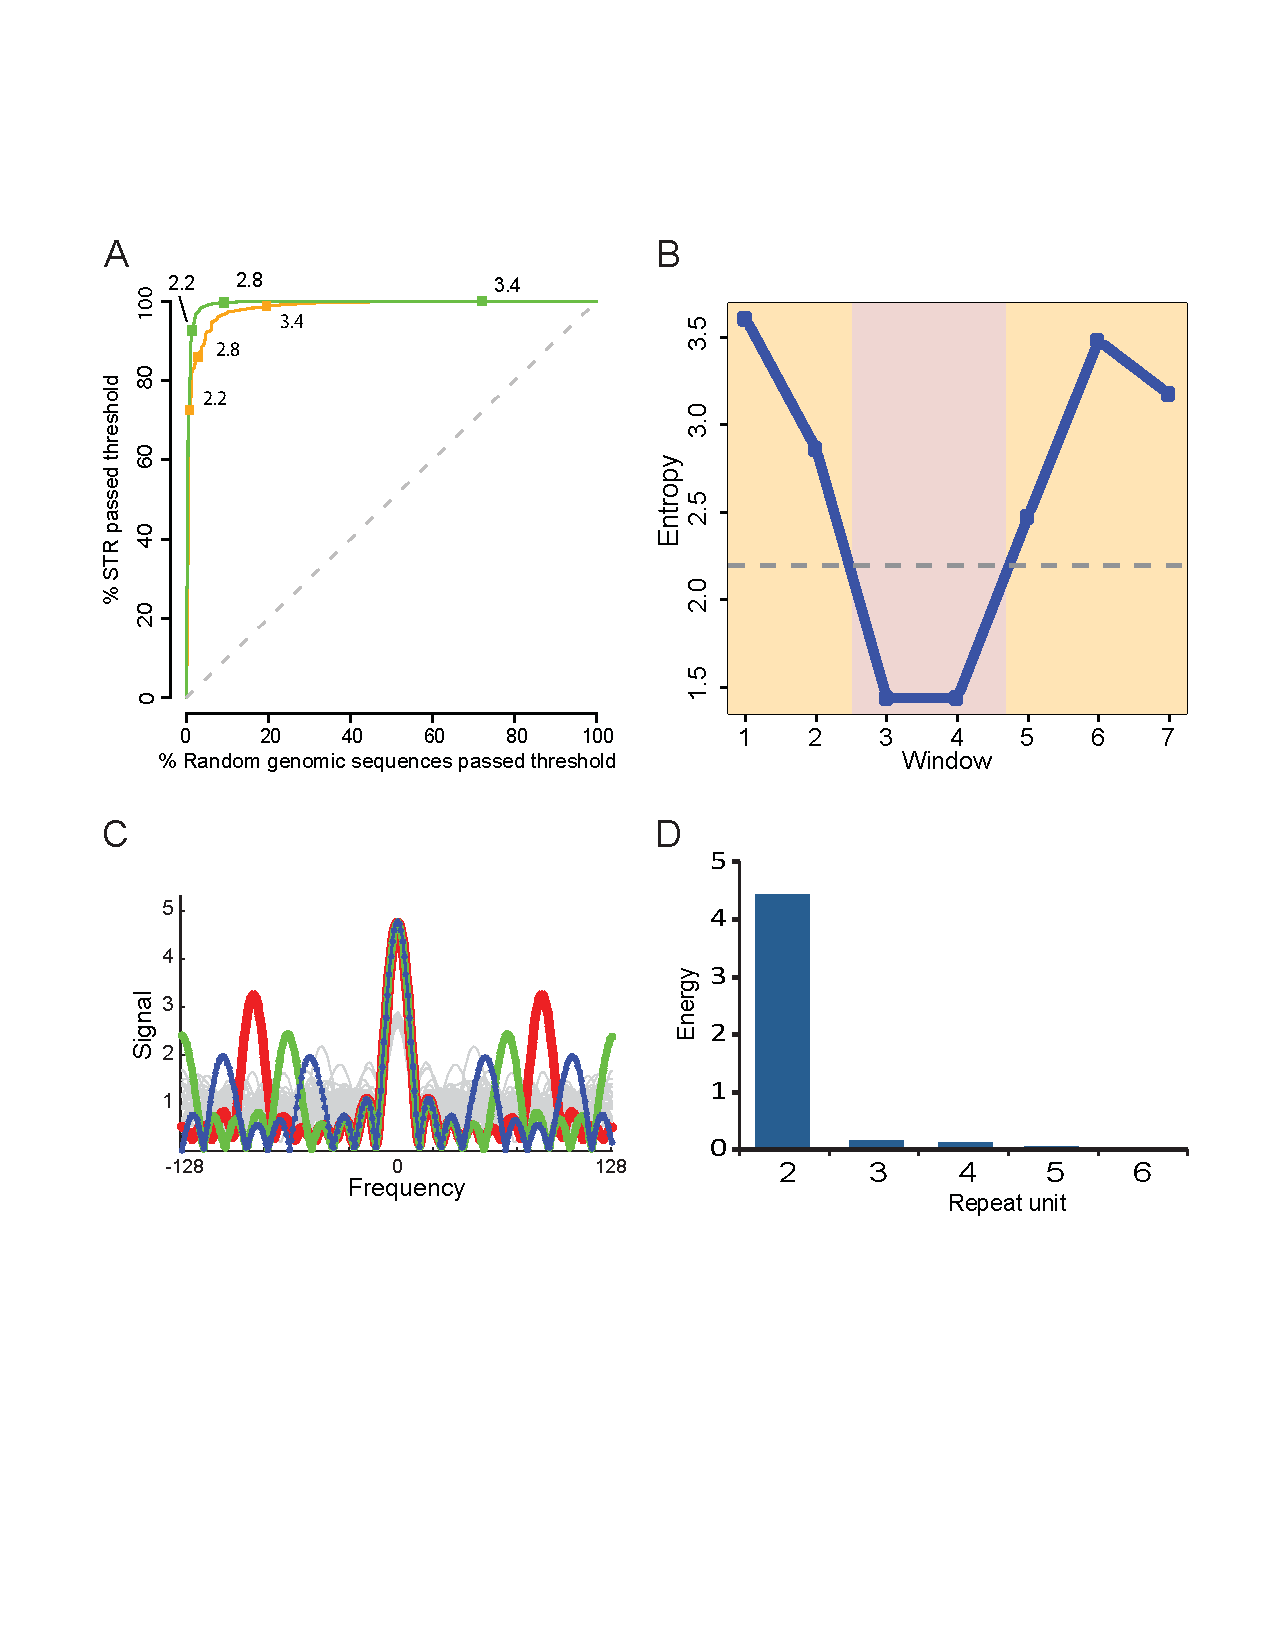
\includegraphics[width=0.65\textwidth]{Figures/Chapter2/SuppFig2.pdf}
\end{figure}
\textbf{Detection of STR containing reads} \textbf{(A) Entropy scores discriminate between STR sequences and random genomic sequences.} The receiver operating curve of the rate of STRs passing the threshold (sensitivity) versus the rate of random genomic sequences passing the threshold (1-specificity). The dinucleotide entropy (green) shows nearly perfect classification and outperforms the mononucleotide entropy (orange). The numbers on the curves denote the corresponding entropy threshold \textbf{(B) Informative reads have a unique signature in entropy analysis.} The dinucleotide entropy score is presented for sliding windows along the STR-containing sequence. The flanking regions (yellow) have a high entropy score, whereas the STR-containing region (pink) exhibits a low score. The dashed line depicts lobSTR's default entropy threshold \textbf{(C) STR periods create distinct signals in the frequency domain.} The normalized spectral response of STR repeats is characterized by distinct harmonics corresponding to the repeat unit size (blue - 5mer, green - 4mer, red - 3mer, gray - random noise) \textbf{(D) Spectral analysis determines the repeat unit length.} The period whose first harmonic shows the maximum energy is chosen as the repeat length. The example displays the normalized energies of periods 2 through 6 of a dinucleotide STR. 

\pagebreak
\subsection{Supplemental Figure 3}

\begin{figure}[h!]
\centering
\label{fig:lobsup3}
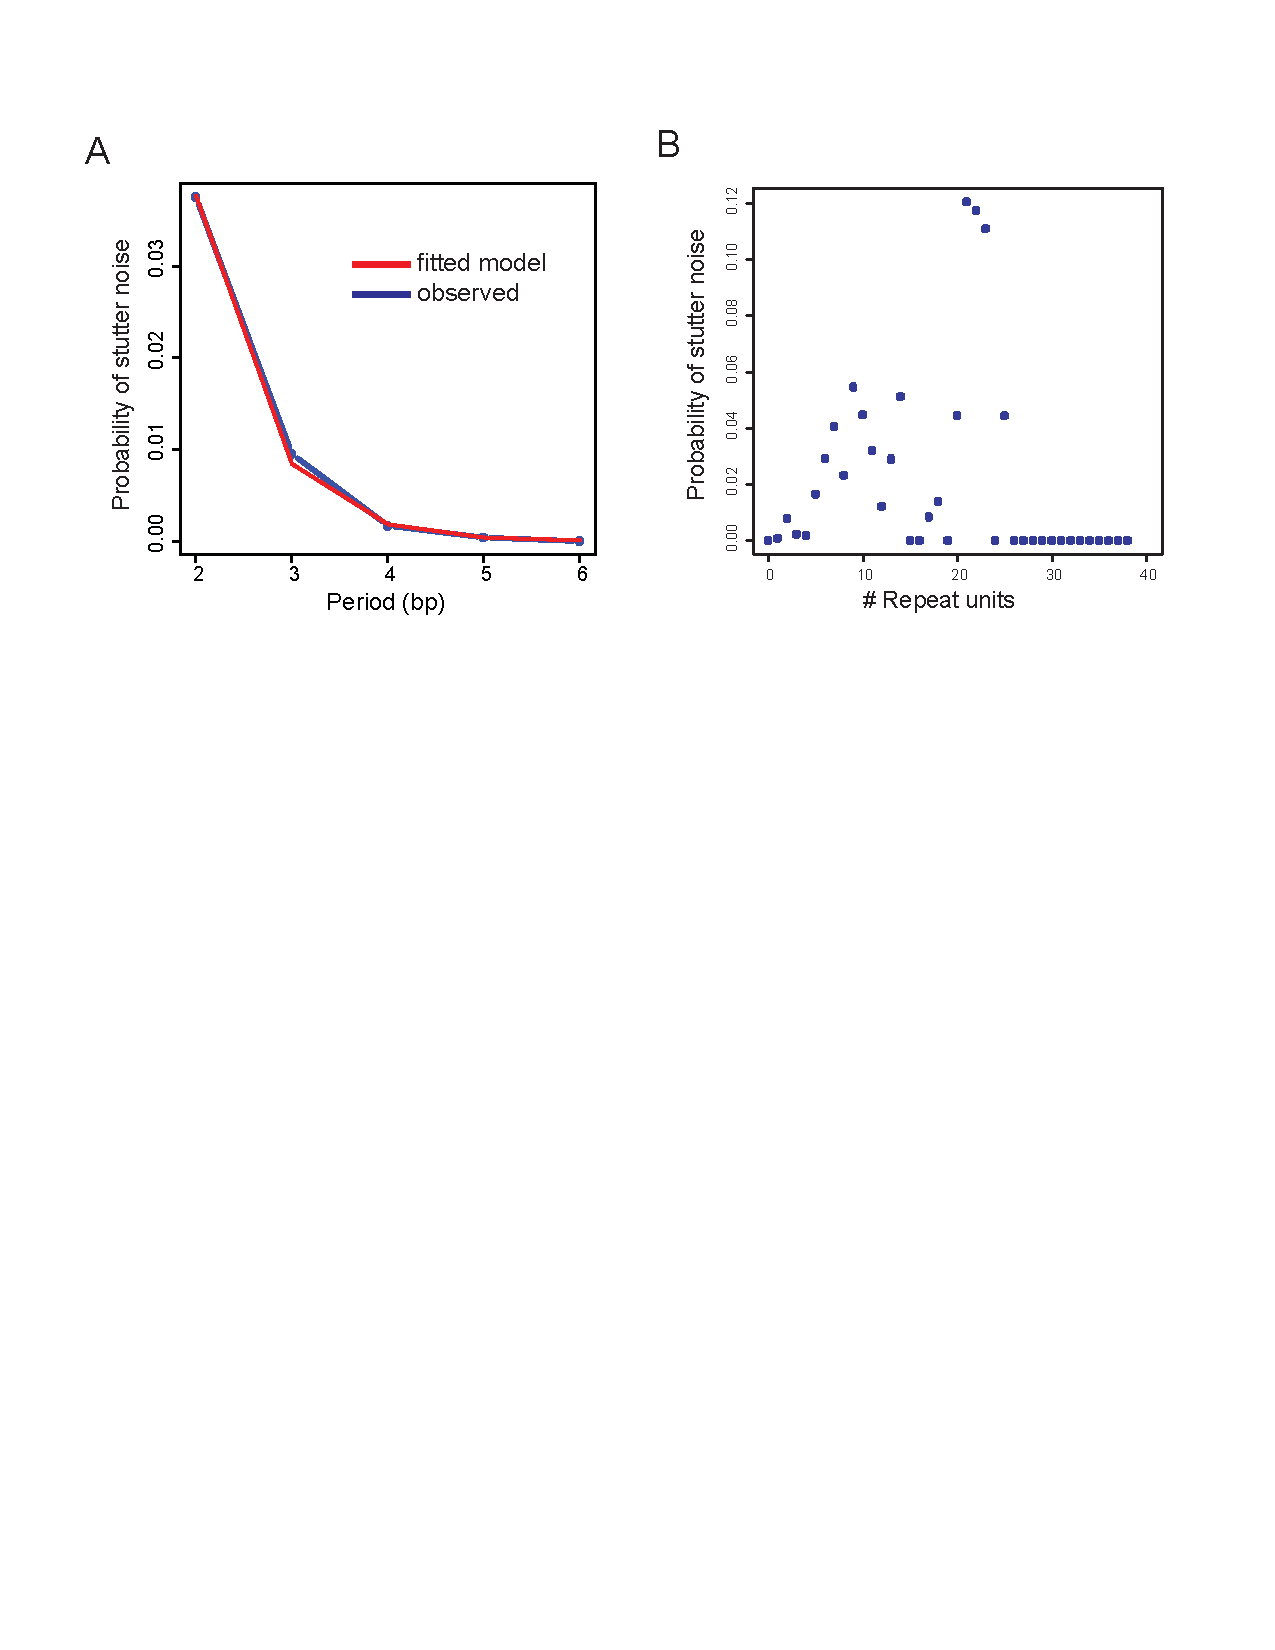
\includegraphics[width=0.7\textwidth]{Figures/Chapter2/SuppFig3.pdf}
\end{figure}
\textbf{The allelotyping step models the likelihood of PCR stutter noise.} \textbf{(A) Stutter noise as a function of STR period.} The probability of PCR stutter noise decreases with period length. Stutter noise (blue) was measured as the percentage of reads from a male sample aligned to sex chromosomes that did not exhibit the mode number of repeat units. We fitted a logistic regression (red) to model noise based on STR period. \textbf{(B) Probability of PCR stutter noise as a function of STR number.} There is no strong association between the STR region length and the stutter noise. 

\pagebreak
\subsection{Supplemental Figure 4}

\begin{figure}[h!]
\centering
\label{fig:lobsup4}
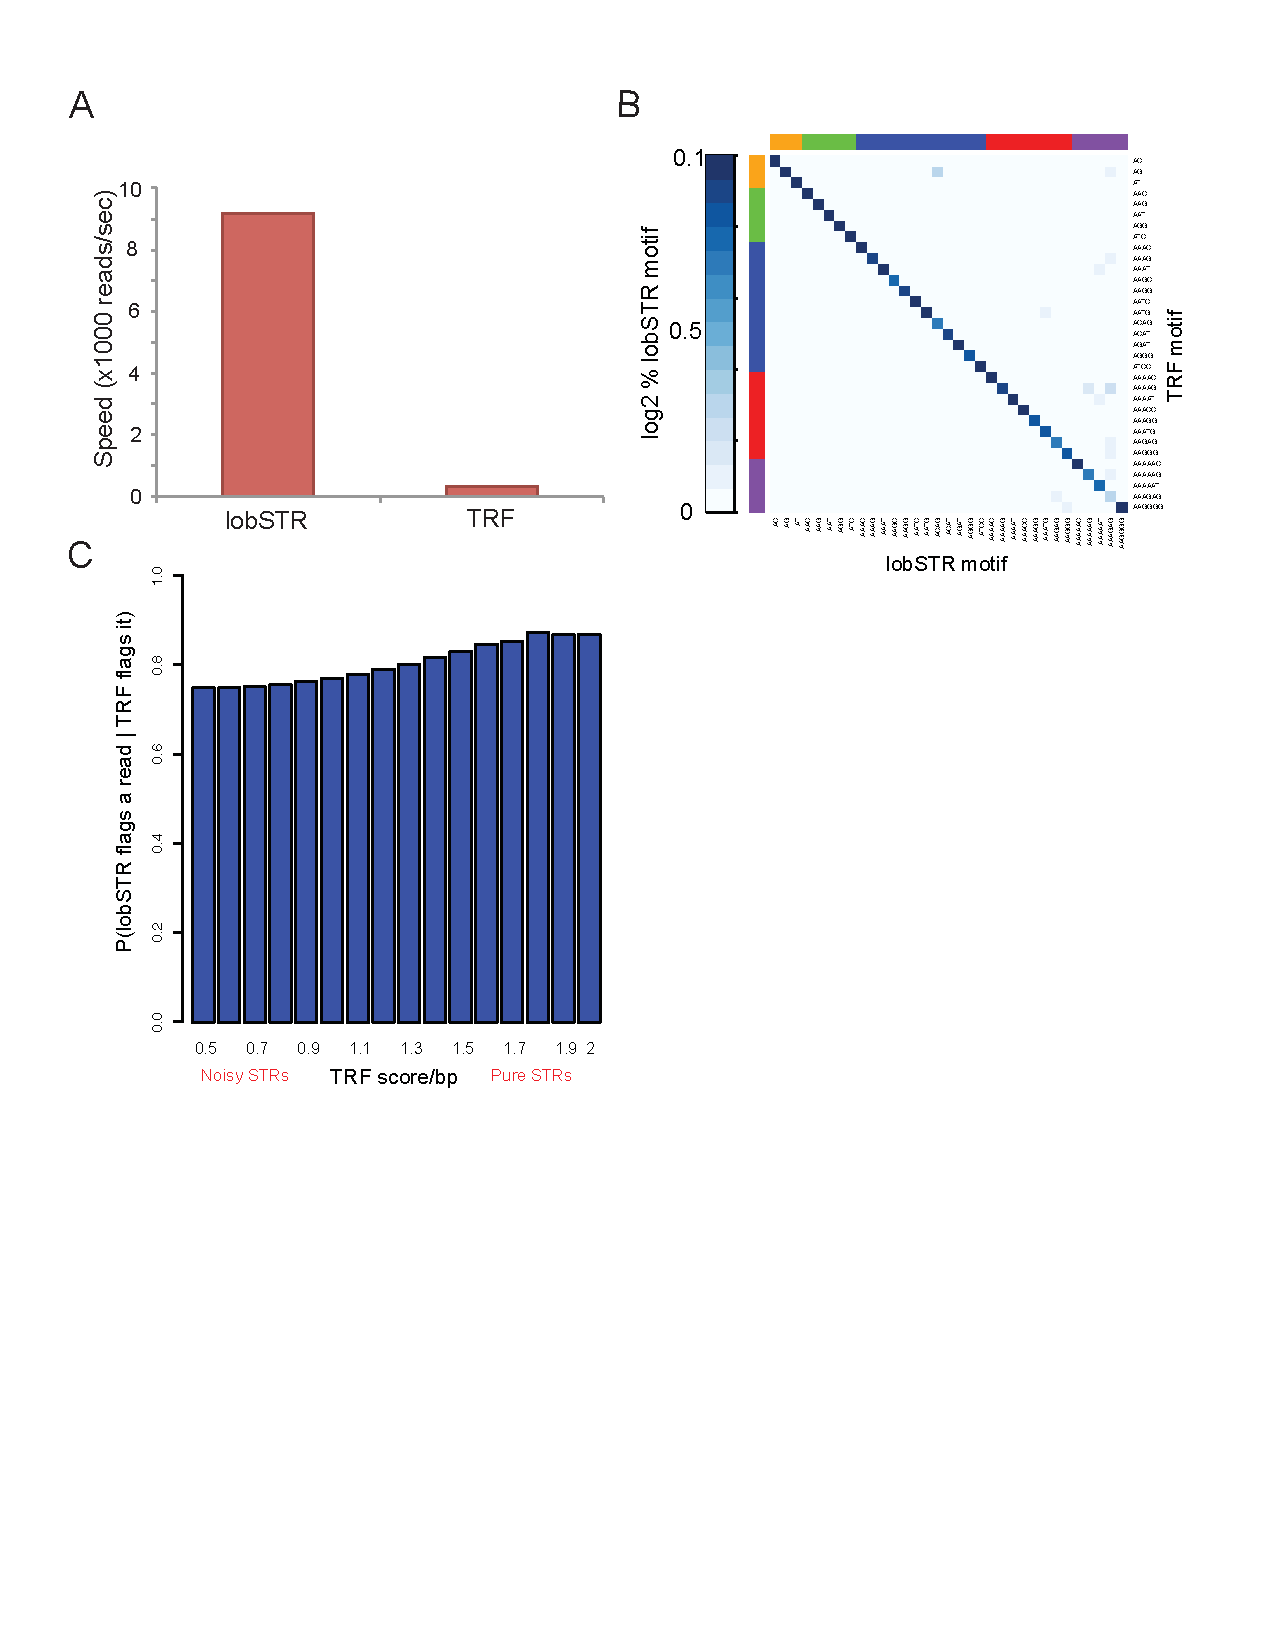
\includegraphics[width=0.7\textwidth]{Figures/Chapter2/SuppFig4.pdf}
\end{figure}
\textbf{Evaluation of the lobSTR sensing step versus TRF} \textbf{(A) lobSTR senses reads 50 times faster than TRF} \textbf{(B) lobSTR motif detection agrees with Tandem Repeat Finder.} In reads where both lobSTR and TRF detect an STR, a comparison of the most represented motifs is shown. Each column is normalized to sum to one, so that values are given in the percentage of instances of a motif detected by lobSTR that were detected as a given motif in TRF. (orange = period 2, green = period 3, blue = period 4, red = period 5, purple = period 6). Overall, lobSTR and TRF agreed in 94\% of the calls \textbf{(C) lobSTR flagging rate for reads that were flagged by TRF as a function of STR purity.} lobSTR flags about 75\% of the reads that were detected from noisy STRs and 85\% of the reads from pure STRs. 

\pagebreak
\subsection{Supplemental Figure 5}

\begin{figure}[h!]
\centering
\label{fig:lobsup5}
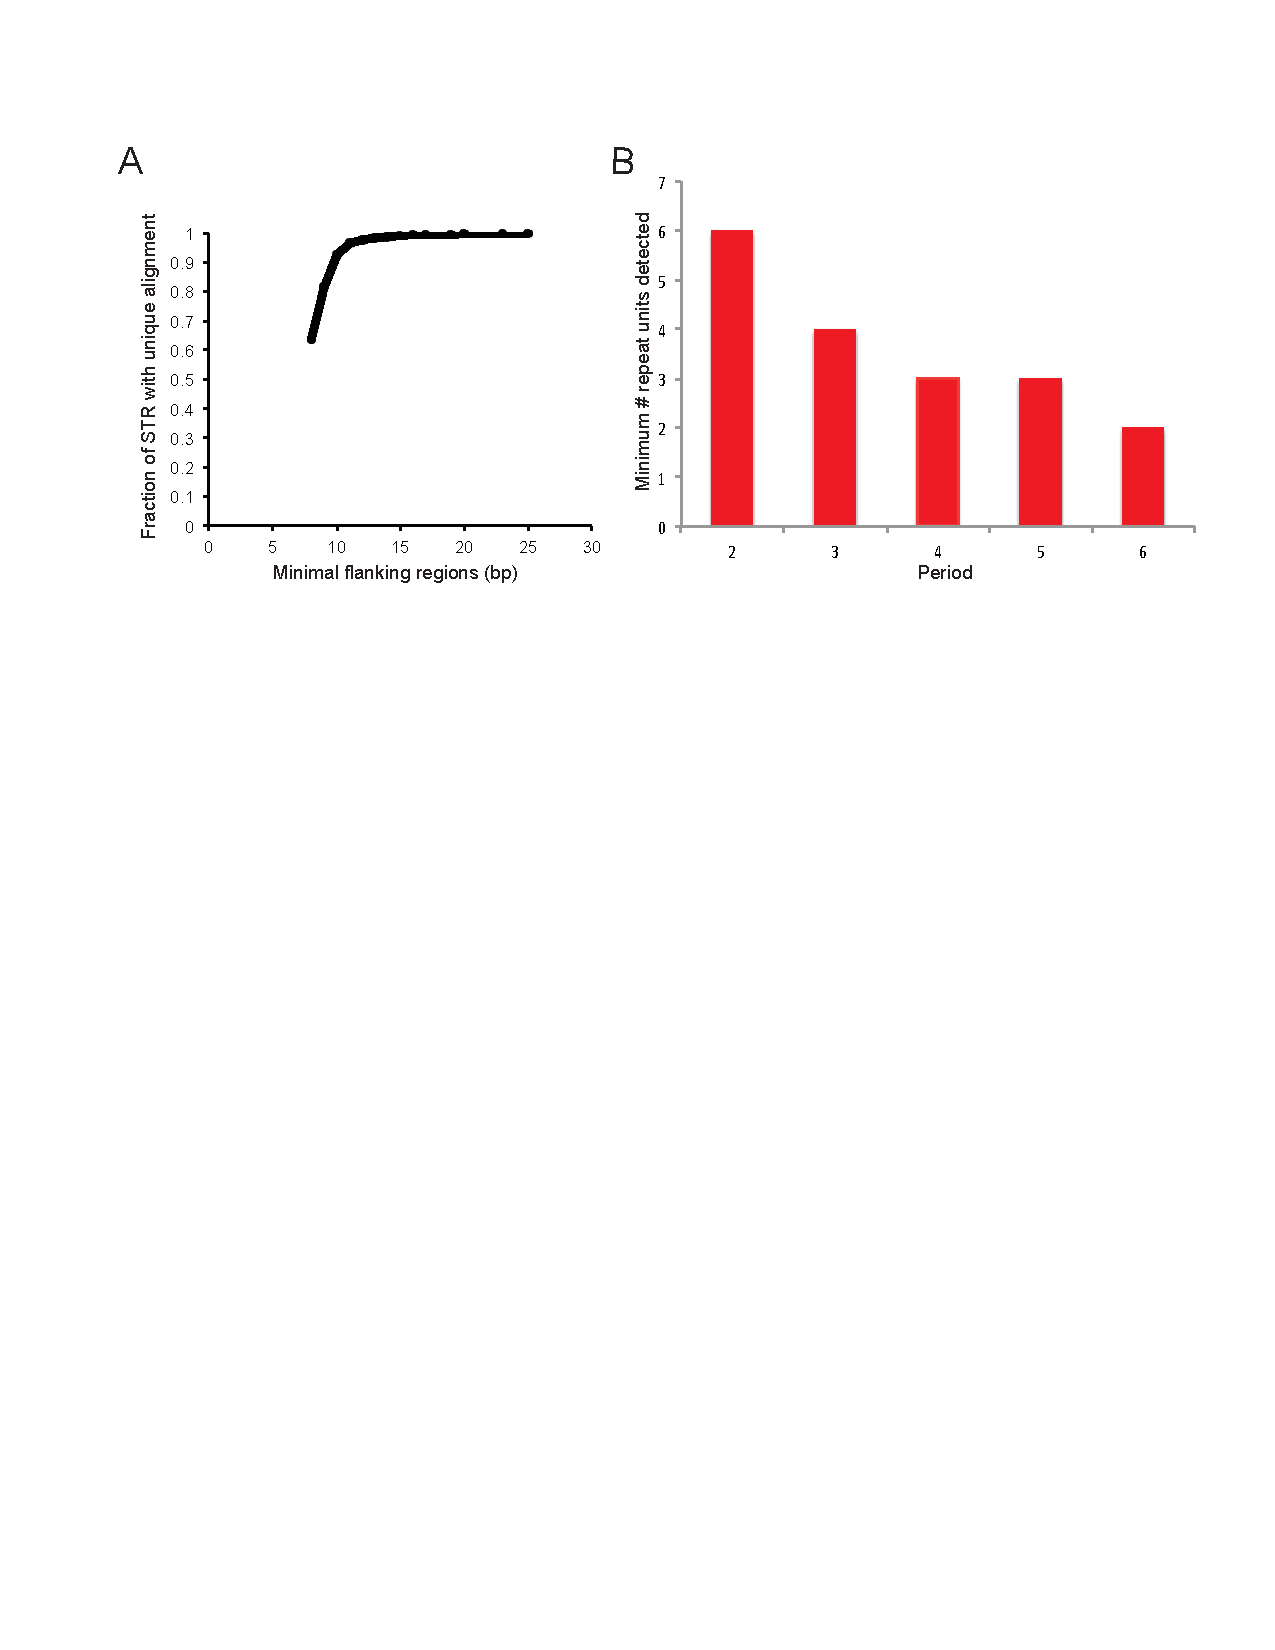
\includegraphics[width=0.7\textwidth]{Figures/Chapter2/SuppFig5.pdf}
\end{figure}
\textbf{Range of STR lengths that lobSTR can process.} lobSTR is able to process STRs with total lengths in the range of 12-84bp from 100bp reads. \textbf{(A) Mappability imposes a lower bound on the size of flanking regions for alignment.} We found that above 9bp upstream and downstream flanking regions, nearly 100\% of STR regions are uniquely aligned \textbf{(B) lobSTR can detect STRs with minimal repeat units.} lobSTR can detect STR regions spanning as few as 12 base pairs. 

\pagebreak
\subsection{Supplemental Figure 6}

\begin{figure}[h!]
\centering
\label{fig:lobsup6}
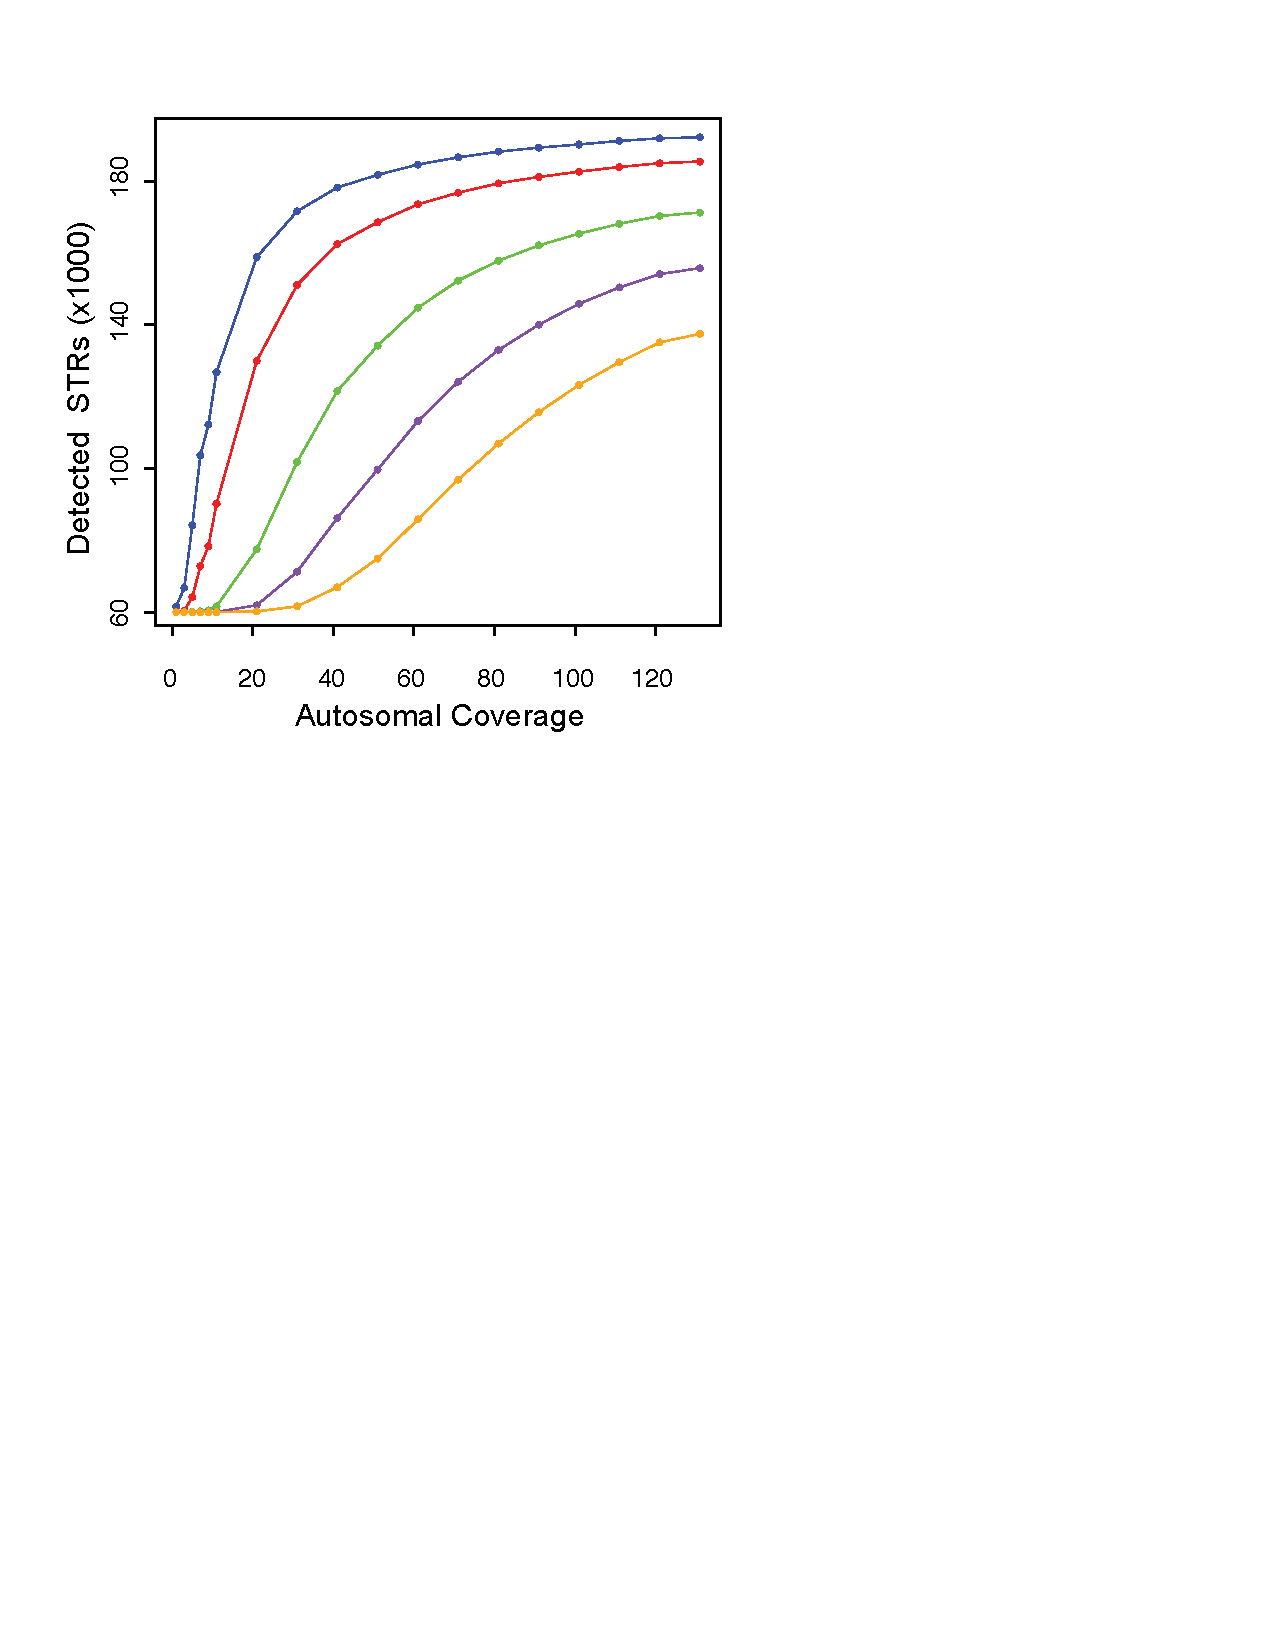
\includegraphics[width=0.7\textwidth]{Figures/Chapter2/SuppFig6.pdf}
\end{figure}
\textbf{Coverage requirements for STR allelotyping.} The number of STR loci at various STR coverage levels (blue - 3x, red - 5x, green - 10x, purple - 15x, orange - 20x) is shown as a function of autosomal genomic coverage. Various coverage levels were simulated by sampling from the aligned reads file of the 126x genome under the assumption that number of aligned STR reads is approximately proportional to genome-wide coverage.

\pagebreak
\subsection{Supplemental Figure 7}
\begin{figure}[h!]
\centering
\label{fig:lobsup7}
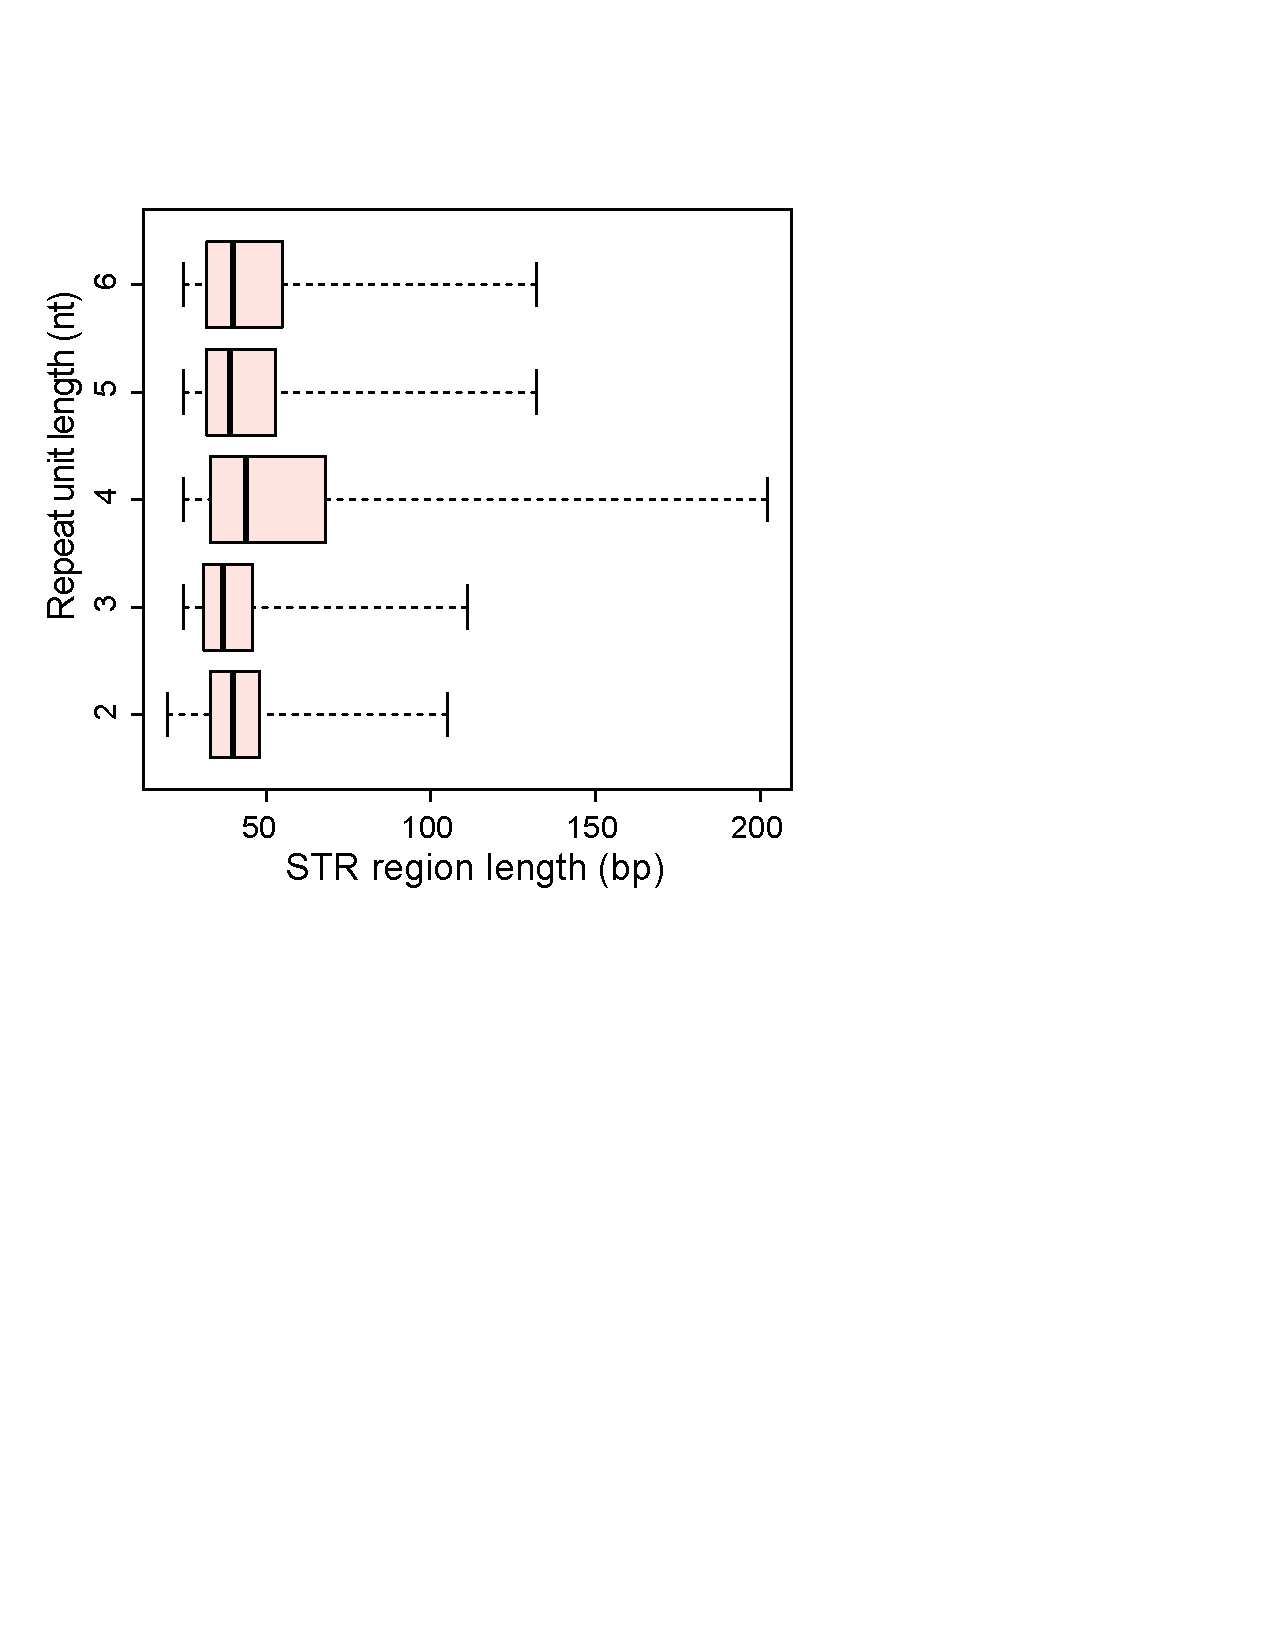
\includegraphics[width=0.7\textwidth]{Figures/Chapter2/SuppFig7.pdf}
\end{figure}
\textbf{Length distribution of STRs.} Most periods have a median STR repeat length (thick black line) of around 40bp. The repeat region total length and length variance increase slightly with increasing repeat period.

\section{Supplemental Tables}

\subsection{Supplemental Table 1}
\label{tab:lobsuptab1}
See the lobSTR website usage page \url{http://lobstr.teamerlich.org/usage.html} for the most up to date lobSTR usage parameters.

\pagebreak

\subsection{Supplemental Table 2}

\begin{table}[h!]
\centering
\label{tab:lobsuptab2}
\begin{tabular}{l l l }
\hline
Genome & Autosomal Coverage & Processing time \\
\hline
HGDP00778 &	5x &	1.3 hours\\
Male individual	& 36x	& 8.5 hours\\
Ajay, et al. &	126x	& 26 hours\\
\hline
\end{tabular}
\caption{\textbf{Processing times of Illumina genomes at various coverage levels.} Processing times as a result of running lobSTR with 25 processors (-p 25).}
\end{table}

\pagebreak

\subsection{Supplemental Table 3}
\begin{table}[h!]
\centering
\label{tab:lobsuptab3}
\begin{tabular}{l l l l l }
\hline
Sample	& Coverage& 	STR Aligned reads	& STRs $\geq$1x	& STRs $\geq$3x\\
\hline
HGDP00456 (Mbuti Pygmy)               & 1.4x & 70,424  & 50,505 & 3,339  \\
HGDP00998 (Karitiana Native American) & 1.3x & 65,236  & 48,481 & 2,553  \\
HGDP00665 (Sardinian)                 & 1.5x & 91,157  & 58,623 & 6,215  \\
HGDP00491 (Bougainville Melanesian)   & 1.7x & 97,398  & 61,463 & 6,523  \\
HGDP00711 (Cambodian)                 & 1.9x & 104,594 & 66,566 & 7,263  \\
HGDP01224 (Mongolian)                 & 1.7x & 93,938  & 61,356 & 5,767  \\
HGDP00551 (Papuan)                    & 1.6x & 94,540  & 61,486 & 6,036  \\
HGDP00521 (French)                    & 5.9x & 184,437 & 91,813 & 17,855 \\
HGDP01029 (San)                       & 7.7x & 192,798 & 93,376 & 18,928 \\
HGDP00542 (Papuan)                    & 5.9x & 118,232 & 72,654 & 7,065  \\
HGDP00927 (Yoruba)                    & 4.8x & 155,136 & 84,828 & 12,774 \\
HGDP00778 (Han)                       & 5.0x & 141,522 & 80,631 & 10,815 \\
\hline
\end{tabular}
\caption{\textbf{HGDP sample coverage and lobSTR results.}}
\end{table}

\pagebreak

\subsection{Supplemental Table 4}
\begin{table}[h!]
\centering
\label{tab:lobsuptab4}
\begin{adjustbox}{width=1\textwidth,height=0.5\textwidth}
\begin{tabular}{l l l l l l l l  }
\hline
Sample & Period & Marker & Refseq (hg18 diff) & Coverage & Converted lobSTR allele$^a$ & Converted HGDP allele$^a$ & Status$^b$ \\ 
\hline
HGDP01029 & 4 & D11S2371 & (TATC)11 & 5 & 0,0   & 0,0   & 2   \\
HGDP01029 & 4 & D12S1300 & (TAGA)12 & 5 & 0,0   & 0,0   & 2   \\
HGDP00521 & 4 & D6S1009  & (TATC)11 & 5 & 1,1   & 1,4   & 1   \\
HGDP01029 & 4 & D2S405   & (TAGA)12 & 5 & -2,-2 & -2,0  & 1   \\
HGDP00778 & 4 & D8S1108  & (TCTA)11 & 4 & 0,0   & 0,0   & 2   \\
HGDP01029 & 4 & D15S818  & (TAGA)10 & 4 & 3,3   & 3,3   & 2   \\
HGDP00551 & 4 & D1S1653  & (TCTA)12 & 4 & -1,0  & -1,0  & 2   \\
HGDP00521 & 4 & D5S2500  & (ATAG)11 & 4 & 0,1   & 0,1   & 2   \\
HGDP00927 & 4 & D10S1426 & (TATC)11 & 4 & 0,2   & 0,2   & 2   \\
HGDP01029 & 4 & D17S1308 & (TGTA)11 (-1)& 4 & -1,-1 & -1,-1 & 2   \\
HGDP00521 & 4 & D17S1308 & (TGTA)11 (-1)& 4 & -1,0  & -1,0  & 2   \\
HGDP00542 & 4 & D17S1308 & (TGTA)11 (-1) & 4 & -1,-1 & -1,-1 & 2   \\
HGDP00927 & 2 & D3S3644  & (AC)16   & 4 & -1,0  & 0,0   & 0.5 \\
HGDP00521 & 2 & D9S1779  & (AC)14   & 4 & 0,0   & -2,-2 & 0   \\
HGDP00521 & 2 & D8S503   & (AC)17   & 4 & 2,4   & 3,6   & 0   \\
HGDP00521 & 2 & D1S2682  & (CA)10   & 3 & 0,10  & 0,10  & 2   \\
HGDP00998 & 4 & D2S427   & (GATA)9  & 3 & 0,0   & 0,0   & 2   \\
HGDP00542 & 4 & D8S1113  & (GGAA)12 & 3 & -6,-6 & -6,-6 & 2   \\
HGDP01029 & 4 & D10S1425 & (GATA)11 & 3 & -5,0  & -5,0  & 2   \\
HGDP01029 & 4 & D7S1824  & (TCTA)11 & 3 & -3,-2 & -3,-2 & 2   \\
HGDP00778 & 4 & D1S3669  & (TATC)10 & 3 & 1,1   & 1,1   & 2   \\
HGDP00711 & 4 & D3S2432  & (AGAT)15 (-3) & 3 & -3,0  & -3,0  & 2   \\
HGDP00491 & 4 & D2S405   & (TAGA)12 & 3 & 0,0   & 0,0   & 2   \\
HGDP00998 & 4 & D16S3253 & (TAGA)9  & 3 & 0,0   & 0,0   & 2   \\
HGDP00998 & 4 & D9S301   & (GATA)15 & 3 & -7,-1 & -7,-1 & 2   \\
HGDP00998 & 4 & D19S586  & (TAGA)12 (+2)& 3 & 1,2   & 1,2   & 2   \\
HGDP00711 & 2 & D15S165  & (AC)21   & 3 & -6,-6 & -6,-6 & 2   \\
HGDP00665 & 2 & D20S103  & (AC)16   & 3 & -1,-1 & -1,-1 & 2   \\
HGDP00456 & 3 & D4S2394  & (ATT)11  & 3 & 0,0   & 0,0   & 2   \\
HGDP00711 & 4 & D11S2371 & (TATC)11 & 3 & 1,1   & 1,1   & 2   \\
HGDP00927 & 4 & D10S1239 & (ATCT)11 & 3 & 0,1   & 0,1   & 2   \\
HGDP00521 & 4 & D14S1434 & (GATA)10 & 3 & 0,0   & 0,0   & 2   \\
HGDP00491 & 4 & D19S591  & (TAGA)10 (-2)& 3 & -1,0  & -1,0  & 2   \\
HGDP00521 & 4 & D19S591  & (TAGA)10 (-2)& 3 & -2,1  & -2,1  & 2   \\
HGDP00542 & 4 & D19S591  & (TAGA)10 (-2) & 3 & -1,0  & -1,0  & 2   \\
HGDP00551 & 4 & D19S591  & (TAGA)10 (-2) & 3 & -2,0  & -2,0  & 2   \\
HGDP01224 & 4 & D19S591  & (TAGA)10 (-2)& 3 & -2,1  & -2,1  & 2   \\
HGDP00927 & 4 & D17S2196 & (AGAT)9 (-2) & 3 & 0,2   & 0,2   & 2   \\
HGDP01029 & 4 & D2S1391  & (ATCT)14 & 3 & -2,0  & -2,0  & 2   \\
HGDP00456 & 3 & D4S2361  & (TTA)13  & 3 & -1,-1 & -1,-1 & 2   \\
HGDP00665 & 4 & D1S1653  & (TCTA)12 & 3 & 0,0   & 0,0   & 2   \\
HGDP01224 & 4 & D1S1653  & (TCTA)12 & 3 & -2,-1 & -2,-1 & 2   \\
HGDP00542 & 4 & D5S2500  & (ATAG)11 & 3 & 0,0   & 0,0   & 2   \\
HGDP00778 & 4 & D10S1426 & (TATC)11 & 3 & 1,1   & 1,1   & 2   \\
HGDP01029 & 4 & D5S2500  & (ATAG)11 & 3 & -2,0  & -2,0  & 2   \\
HGDP00456 & 4 & D17S1298 & (TGAA)8  & 3 & 0,0   & 0,0   & 2   \\
HGDP00927 & 4 & D17S1298 & (TGAA)8  & 3 & 3,3   & 3,3   & 2   \\
HGDP00542 & 4 & D19S254  & (AGAT)13 (-6) & 3 & -1,1  & -1,1  & 2   \\
HGDP00711 & 2 & D1S2682  & (CA)10   & 3 & 0,0   & 0,10  & 1   \\
HGDP00998 & 4 & D5S1457  & (ATAG)9  & 3 & 0,0   & 0,1   & 1   \\
HGDP00521 & 2 & D20S103  & (AC)16   & 3 & 2,2   & -1,2  & 1   \\
HGDP00998 & 4 & D20S482  & (TCTA)14 & 3 & 0,0   & 0,1   & 1   \\
HGDP01224 & 3 & D9S910   & (ATA)14  & 3 & -7,-7 & -7,-7 & 1   \\
HGDP01224 & 4 & D11S2363 & (TATC)14 & 3 & -1,-1 & -1,9  & 1   \\
HGDP00711 & 4 & D19S591  & (TAGA)10 (-2) & 3 & -1,-1 & -1,0  & 1   \\
HGDP00927 & 2 & D18S1390 & (TG)18   & 3 & -1,0  & -2,-1 & 0.5 \\
HGDP00778 & 2 & D8S503   & (AC)17   & 3 & 2,3   & 3,3   & 0.5 \\
HGDP00778 & 4 & D12S1300 & (TAGA)12 & 3 & 2,4   & 2,2   & 0.5 \\
HGDP00491 & 2 & D9S1779  & (AC)14   & 3 & 0,9   & -1,6  & 0  \\
\hline
\end{tabular}
\end{adjustbox}
\caption{\textbf{Comparison of lobSTR allelotype calls to the CEPH-HGDP results.} Differences between the RefSeq sequence and hg18 are indicated in parentheses. $^a$Converted allelotypes given in number of repeat units different from the reference. $^b$Status: 2 = both alleles called correctly, 1 = one allele of a heterozygous locus called correctly, 0.5 = one allele called correctly and one incorrectly, 0 = no correct alleles called.}
\end{table}

\pagebreak

\subsection{Supplemental Table 5}
\begin{table}[h!]
\centering
\label{tab:lobsuptab5}
\begin{adjustbox}{width=1\textwidth}
\begin{tabular}{l l l l l l l l  }
\hline
Genome (platform) & Coverage& Input reads & Avg. Read length & STR Aligned reads / Mbp input& \% Non-unit Reads$^*$ &	STRs $\geq$1x	STRs $\geq$3x \\
\hline
Venter (Sanger)        & 7.5x  & 12.5M & 996 & 24.78 & 7.30\%  & 127,017 & 41,261  \\
Watson (454)           & 7.4x  & 75M   & 183 & 10.41 & 25.00\% & 83,079  & 25,488  \\
Moore (IonTorrent)     & 10.6x & 860M  & 261 & 0.79  & 43.50\% & 65,758  & 13,413  \\
Ajay, et al (Illumina) & 126x  & 14B   & 100 & 4.36  & 8.00\%  & 180,309 & 167,175 \\
\hline
\end{tabular}
\end{adjustbox}
\caption{\textbf{lobSTR performance on four sequencing platforms.}  $^*$Reads differing by a non-integer number of copies of the STR motif from the reference. (M = million, B = billion). }
\end{table}

\pagebreak

\subsection{Supplemental Table 6}
\begin{table}[h!]
\centering
\label{tab:lobsuptab6}
\begin{tabular}{l l l}
\hline
Repeat unit size & \# STR loci & Percentage \\
\hline
2 &	106,457 &	44\% \\
3&	17,383	&7\% \\
4	&70,847&	30\% \\
5	&28,746	&12\% \\
6	& 16,626	& 7\% \\
Total &	240,059	& 100\% \\
\hline
\end{tabular}
\caption{\textbf{STR reference repeat unit size distribution.}}
\end{table}

\pagebreak

\subsection{Supplemental Table 7}
% TODO
\begin{table}[h!]
\centering
\label{tab:lobsuptab7}
\begin{tabular}{l l}
\hline
Repeat unit & \# STR loci \\
\hline
AC	& 66,992\\
AT	& 25,661\\
AAAT &	20,319\\
AG	& 13,778\\
AAAG	& 12,553\\
AAAAC &	10,015 \\
AAGG	 & 9,862\\
AAAC	& 8,842\\
AGAT	& 7,127\\
AAAAT	& 7,115\\

\hline
\end{tabular}
\caption{\textbf{Most frequent reference STR repeat units.}}
\end{table}


%% TODO figures/tables and legends